% =====================================================================
%  ReVar3R -- comprehensive two-column preprint
%  (CVPR main paper + supplementary merged into one expanded document)
%  Build: pdflatex preprint -> bibtex preprint -> pdflatex preprint x2
%  The CVPR main.tex / supplementary.tex are left untouched.
% =====================================================================
\documentclass[10pt,twocolumn,letterpaper]{article}

\usepackage{cvpr}                  % CVPR two-column style, camera-ready (no review banner / line numbers)
\input{preamble}                   % microtype
\input{macros}                     % \trustr/\ause/\best macros + float tuning (twocolumn-aware)

\usepackage{amsmath}
\usepackage{amssymb}
\usepackage{amsfonts}
\usepackage{pifont}                % \ding cross/check glyphs (status table)
\usepackage{graphicx}
\graphicspath{{figures/}}
\usepackage{subcaption}
\usepackage{dblfloatfix}            % robust placement of full-width (starred) floats in two-column
\setcounter{totalnumber}{12}

% hyperref last, then cleveref (in arxiv_compat)
\definecolor{linknavy}{rgb}{0.10,0.30,0.55}
\usepackage[pagebackref,breaklinks,colorlinks,allcolors=linknavy]{hyperref}
\input{arxiv_compat}               % cleveref (after hyperref) + math operators; abbrevs already in cvpr.sty

\def\paperID{}
\def\confName{Preprint}
\def\confYear{2026}

\title{ReVar3R: Training-Free Calibrated Uncertainty for Frozen Feed-Forward 3D Foundation Models}
\author{Anonymous}

\begin{document}
\maketitle

\begin{abstract}
Frozen feed-forward 3D foundation models (\vggt, \pii, \mastr) turn a few images into dense
point maps in one forward pass, and emit a per-pixel \emph{confidence} channel that downstream
systems increasingly trust. We show this channel is an unreliable uncertainty: it is weak and
\emph{uneven} in-distribution (e.g.\ VGGT/7-Scenes \ause---area under the sparsification-error curve, lower is better---$0.71$ vs.\ $0.84$ for random, Spearman
only $+0.07$) and, crucially, \emph{collapses} where it is most needed --- its correlation with
true error falls to $\approx\!0$ out-of-distribution (ETH3D, all three models) and turns
\emph{negative} on several cells (VGGT/BlendedMVS $-0.12$, MASt3R/DTU $-0.10$). We propose
\trustr, a training-free, inference-only estimator: run the frozen model $N{=}5$ times under
geometry-preserving perturbations, \emph{robustly register each run's point map into a common
frame before measuring per-point variance} (Umeyama${+}$IRLS), calibrate with isotonic
regression, and fuse the two perturbation estimators \emph{together with the model's own
confidence} by a held-out rank-weighting. Across \textbf{three models
and four datasets (12 cells)}, \trustr\ significantly reduces \ause\ in \textbf{9} (by
$3\text{--}36\%$), \emph{including the out-of-distribution set for all three architectures}; the
wins are \emph{predicted} by where the built-in confidence is mis-calibrated, and the three
non-wins are precisely the BlendedMVS cells (the models' own training corpus), where it is
already well calibrated --- a mechanistic coupling
stronger than blanket superiority. A central finding is that \trustr\ \emph{matches or beats an
MLP probe trained on the model's own frozen features} on every dataset, indicating the usable
signal is \emph{consistent with} epistemic input-sensitivity rather than something static in the representation. Using
\trustr\ to filter multi-view fusion yields near-oracle cloud accuracy in-distribution while
preserving far more completeness. We report honest negatives (no novel-view-synthesis gain; a
null out-of-distribution fusion gain; one falsified hypothesis). Everything runs on a single
16\,GB consumer GPU.
\end{abstract}


\section{Introduction}
\label{sec:intro}

Feed-forward 3D foundation models have, since 2024, become the dominant way to recover geometry
from images. Where classical photogrammetry needed many overlapping photographs, careful camera
calibration, and a slow two-stage optimization (structure-from-motion for the cameras, then
multi-view stereo for dense geometry), these models regress geometry \emph{directly} from raw
pixels. DUSt3R-style models~\cite{dust3r,mast3r} predict a per-pixel \emph{point map}---for every
pixel, the $(x,y,z)$ coordinate of the surface it sees, expressed in one shared coordinate
frame---and recent transformers scale this to many views and unify depth, camera pose and point
maps in a single forward pass~\cite{vggt,fast3r,cut3r,pi3}. \vggt~\cite{vggt} won the CVPR'25 Best
Paper Award; \pii~\cite{pi3} made the architecture permutation-equivariant (its output does not
depend on the order in which the images are fed). These models are released openly, run in seconds
on a single GPU, and their entire value lies in \emph{downstream use}: multi-view fusion into a
clean point cloud, 3D Gaussian Splatting initialization~\cite{instantsplat,gsplat}, SLAM and
robotics. Every such consumer faces the same question before it can act: \emph{which of the
predicted points should it trust?}

\begin{figure*}[tbp]
  \centering
  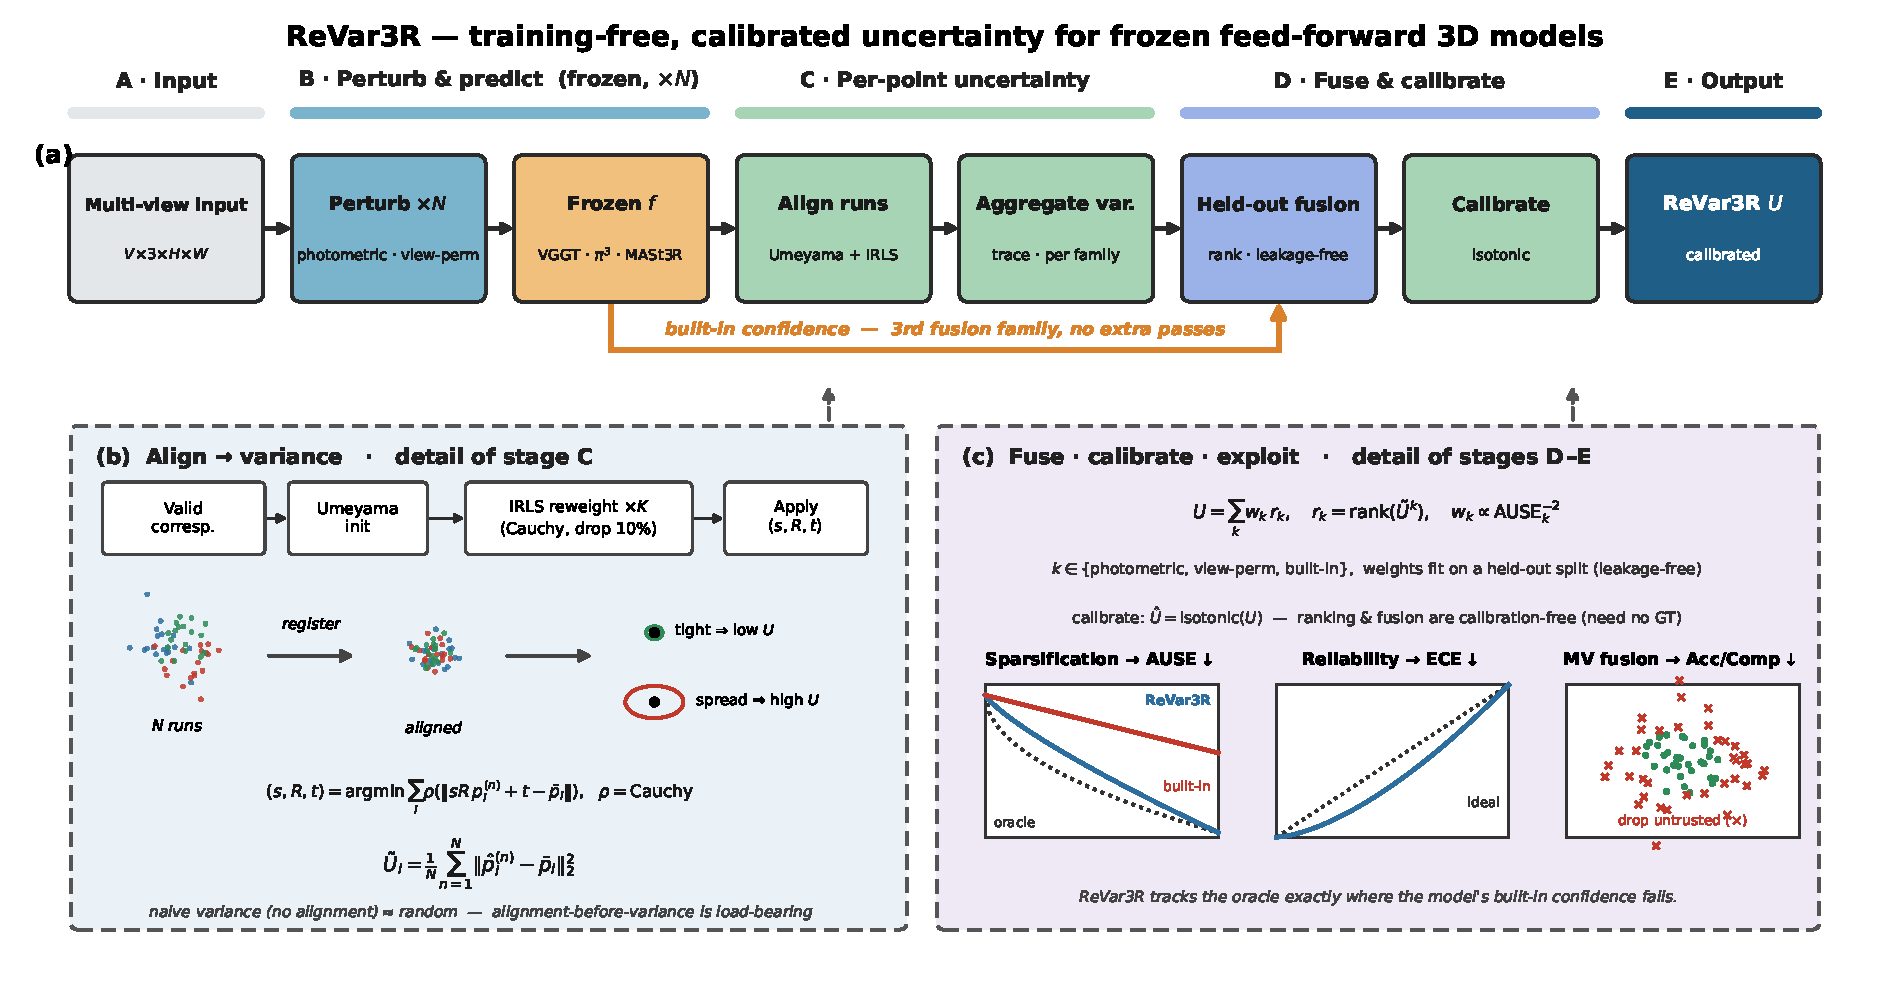
\includegraphics[width=\textwidth]{pipeline.pdf}
  \caption{\textbf{\trustr\ overview.} \emph{When the model's own confidence lies, perturbation
  tells the truth.} (a) The training-free pipeline: run the \emph{frozen} model $N$ times under
  geometry-preserving perturbations, robustly align each run into a common frame, take per-point
  trace-variance, fuse the two perturbation families \emph{together with} the model's own built-in
  confidence via held-out, leakage-free weights, and calibrate. (b) The alignment-before-variance step (our technical crux), with the
  robust-alignment and trace-variance equations. (c) The held-out fusion and isotonic-calibration
  equations, and how the uncertainty $U$ is evaluated and exploited downstream.}
  \label{fig:pipeline}
\end{figure*}

These models do emit a per-pixel \emph{confidence}, but it is trained as a reconstruction
loss-weight, not a calibrated uncertainty---the 3D analogue of softmax mis-calibration~\cite{guo}.
A 2025 survey~\cite{survey3d} explicitly names uncertainty quantification for this model family
\emph{``critical and underexplored.''} We give the first systematic evidence of how unevenly the
built-in confidence behaves: it is weak in-distribution---near-random for some model/dataset pairs
(VGGT/7-Scenes Spearman $+0.07$)---and \textbf{collapses where reliability matters most}: its
correlation with error falls to $\approx0$ out-of-distribution (ETH3D, all three models) and turns
\emph{negative} on several in-distribution cells (VGGT/BlendedMVS $-0.12$, MASt3R/DTU $-0.10$). A
signal that flat-lines or inverts under the very shift where reliability matters is worse than useless.

We propose \trustr, a \emph{training-free} estimator that obtains a calibrated per-point
uncertainty from a \emph{frozen} model by measuring its \emph{disagreement with itself} under
small, geometry-preserving input perturbations (photometric jitter and input-view
permutation/subsetting). The key technical subtlety, absent in 2D test-time-augmentation
uncertainty~\cite{ayhan,ttaaleatoric}, is that each perturbed run expresses geometry in its own
gauge: we therefore \emph{robustly register every run into a common frame before measuring
variance} (Umeyama~\cite{umeyama} + IRLS), then take per-point trace-variance, isotonic-calibrate,
and fuse the two estimators by held-out rank-weighting. The estimator needs $\le 10$ forward
passes and runs on a single 16\,GB GPU.

Across \vggt, \pii\ and \mastr\ on four datasets (7-Scenes, DTU, BlendedMVS, ETH3D), \trustr\
significantly reduces \ause\ in \textbf{9 of 12} model$\times$dataset cells (by $3\text{--}36\%$,
paired Wilcoxon)---\emph{including the OOD set for all three architectures, where the built-in
confidence collapses}. The wins are \emph{predicted} by where the confidence is mis-calibrated and
the non-wins are exactly the BlendedMVS cells (the models' training corpus, where the confidence is
already well-calibrated)---a mechanistic coupling, not blanket superiority.
Strikingly, \trustr\ matches or beats an MLP \emph{trained} on the model's own frozen features,
which tells us the usable reliability signal is \emph{epistemic input-sensitivity}, only visible
when the model is actually re-run, rather than a static function of one forward pass. We make the
following contributions:

\begin{itemize}[leftmargin=1.2em,itemsep=1pt,topsep=2pt]
\item \textbf{C1 (a failure mode, characterized).} The first systematic evidence that the built-in
confidence of frozen 3D foundation models is an \emph{uneven} uncertainty---weak in-distribution and
\emph{collapsing} ($\rho{\approx}0$) or \emph{anti-correlated} ($\rho<0$) where reliability matters
most---across three models and four datasets (\Cref{sec:rq1}).
\item \textbf{C2 (alignment-before-variance).} A training-free estimator whose crux is robust
similarity registration of each perturbed run before per-point variance. This is not an engineering
detail but the conceptual core: in 3D each run expresses geometry in its own gauge, so \emph{naive}
perturbation variance is near-random ($0.72$ vs.\ $0.50$ \ause)---registration is what turns
self-disagreement into a usable signal, and the ablation shows it is the single largest contributor
(\Cref{sec:method,sec:exp}).
\item \textbf{C3 (the epistemic insight).} \trustr\ matches/beats a probe trained on the model's
frozen features, evidence that the signal is epistemic input-sensitivity, not in the static
features (\Cref{sec:exp}).
\item \textbf{C4 (a calibrated benchmark + utility).} A reproducible single-GPU protocol
(\ause/\aurg/Spearman/\ece\ + fused-cloud Accuracy/Completeness), a near-oracle multi-view-fusion
utility, and \emph{honest negatives} (no NVS gain; a falsified architectural hypothesis).
\end{itemize}

\noindent\textbf{Paper organization.} \Cref{sec:questions} states the research questions, hypotheses,
and novelty; \Cref{sec:primer} fixes background and notation; \Cref{sec:rq1} documents the
confidence-collapse failure mode; \Cref{sec:method} develops the method; \Cref{sec:exp} and
\Cref{sec:ablations} present the results and ablations; and \Cref{sec:discussion} discusses scope and
limitations.

\section{Research questions, hypotheses, and novelty}
\label{sec:questions}

Feed-forward 3D models ship a per-pixel confidence channel, but its reliability as an uncertainty
estimate has not been examined systematically. We ask whether that channel can be trusted and, where
it cannot, whether a better per-point uncertainty can be obtained \emph{without retraining the model}.
Stated precisely, the goal is:

\begin{quote}
Given a \emph{frozen, pretrained} feed-forward 3D model $f$ and a set of input images, produce a
per-point uncertainty map $U$ over $f$'s predicted geometry such that $U$ is \textbf{(a)} better
correlated with true geometric error than the model's built-in confidence, \textbf{(b)}
well-calibrated, and \textbf{(c)} useful---using $U$ to filter or weight points measurably improves
a downstream task---all \emph{without any additional training of $f$} and within a
single-consumer-GPU budget.
\end{quote}

\subsection{Research questions and hypotheses}
\label{sec:rqs}

We organize the paper around four research questions, each with the hypothesis we set out to test.

\begin{description}[leftmargin=1.4em,itemsep=3pt,topsep=3pt]
\item[RQ1 (quality of the status quo).] \emph{How well does the built-in confidence of a feed-forward
3D model predict its actual geometric error?}\\
\textbf{H1:} the built-in confidence is substantially mis-calibrated and only weakly rank-correlated
with true error, leaving clear headroom for a better signal. (Answered in \Cref{sec:rq1}.)

\item[RQ2 (a training-free estimator).] \emph{Can perturbation-based self-disagreement---running the
frozen model under geometry-preserving input perturbations and measuring how much it disagrees with
itself---yield uncertainty better than the built-in confidence?}\\
\textbf{H2:} yes; the variance of $f$'s predictions under perturbation, \emph{after} the runs are
aligned into a common coordinate frame, beats the built-in confidence on sparsification and
calibration. (Answered in \Cref{sec:exp}.)

\item[RQ3 (architecture and uncertainty).] \emph{Does the architectural difference between
reference-view-dependent models (\vggt, \mastr) and permutation-equivariant models (\pii) manifest
as measurable differences in which perturbation is most informative?}\\
\textbf{H3:} input-view permutation disagreement is a \emph{stronger} signal for the
reference-dependent \vggt\ than for the permutation-equivariant \pii. (Answered---and
\emph{falsified}, instructively---in \Cref{sec:exp} and Appendix~\ref{app:negatives}.)

\item[RQ4 (downstream utility).] \emph{Does uncertainty-guided point filtering or weighting improve a
real downstream task?}\\
\textbf{H4:} initializing or fusing 3D from uncertainty-filtered points yields better geometry/views
than using the raw output or built-in-confidence filtering. (Answered with a \emph{mixed} verdict in
\Cref{sec:exp} and \Cref{sec:ablations}: a clear win for multi-view fusion, a null result for
novel-view synthesis.)
\end{description}

\subsection{What is novel}
\label{sec:novelty}

\trustr's novelty is \emph{not} ``uncertainty estimation'' in general---that is a mature field. It is
the specific, previously-empty intersection of four things.

\begin{enumerate}[leftmargin=1.5em,itemsep=2pt,topsep=2pt]
\item \textbf{First systematic treatment of uncertainty for the feed-forward 3D
foundation-model family} (DUSt3R\,$\rightarrow$\,\vggt\,$\rightarrow$\,\pii). Prior uncertainty work
targets monocular depth~\cite{poggi}, optical flow~\cite{ilg}, or classification---not multi-view
point-map regression from these models. The field's own survey~\cite{survey3d} flags this as open,
and the adjacent methods we are aware of train a new head and are concurrent (an evidential
head~\cite{trust3r_evidential}, an automated-capture module~\cite{auto3r}, 4D-specific
priors~\cite{robust4d}).
\item \textbf{A training-free estimator} that requires zero modification or retraining of the base
model. It therefore transfers across DUSt3R/\mastr/\vggt/\pii\ and to \emph{future} models, and runs
on one consumer GPU.
\item \textbf{The alignment-before-variance insight}, which is genuinely 3D-specific. In 2D,
test-time-augmentation variance can be read off directly; in 3D, each run expresses geometry in its
own arbitrary frame (the ``gauge,'' \Cref{sec:primer}), so the runs must be \emph{robustly
registered before} variance is even meaningful. We show this step is the single largest contributor
to the signal, not an implementation detail.
\item \textbf{A benchmark, a calibration protocol, and a downstream-utility study in one paper}---
turning ``here is a number'' into ``here is a trustworthy, useful number, proven on standard data
with honest negatives.''
\end{enumerate}

\noindent\textbf{Contrast with the closest neighbours.} The base models' \emph{built-in confidence}
is a learned loss-weight, not a calibrated uncertainty; we beat it and explain when. \emph{Test-time
augmentation for uncertainty}~\cite{ayhan,ttaaleatoric} is established for 2D
classification/segmentation but was never formulated for 3D point maps, which additionally require
cross-prediction geometric alignment. \emph{Deep ensembles}~\cite{ensembles} and
\emph{MC-dropout}~\cite{mcdropout} need multiple trained models or dropout layers---neither available
for a single frozen released checkpoint---whereas we perturb one frozen model at inference.

\subsection{Outcome of the hypotheses}
\label{sec:hyp-status}

Each hypothesis's outcome is summarized in \Cref{tab:hyp-status}. Reporting the falsified hypothesis
(H3) and the null downstream result (part of H4) is a deliberate part of the contribution: the value
of a reliability study is undercut if it hides its own unreliable findings.

\begin{table*}[t]
\centering\small
\begin{tabular}{@{}llll@{}}
\toprule
Hyp. & Claim (abbreviated) & Verdict & Where \\
\midrule
H1 & built-in confidence weak / mis-calibrated; headroom exists & Supported & \Cref{sec:rq1} \\
H2 & perturbation variance (after alignment) beats confidence & Supported (9/12) & \Cref{sec:exp} \\
H3 & view-permutation stronger for \vggt\ than \pii & \textbf{Falsified} (reversed) & Appendix~\ref{app:negatives} \\
H4 & uncertainty-guided downstream gain & Mixed: fusion \checkmark, NVS \ding{55} & \Cref{sec:exp}, \Cref{sec:ablations} \\
\bottomrule
\end{tabular}
\caption{Where each hypothesis stands. H1/H2 are supported; H3 is falsified in an informative way
(the permutation signal is in fact \emph{stronger} on \pii, via leave-one-out subsetting rather than
shuffling); H4 is mixed---a near-oracle multi-view-fusion gain but no novel-view-synthesis gain.}
\label{tab:hyp-status}
\end{table*}

\section{Background and preliminaries}
\label{sec:primer}

We fix the concepts and notation the paper relies on: the point-map output of feed-forward models,
the gauge ambiguity that makes 3D uncertainty non-trivial, the epistemic/aleatoric distinction, and
the sparsification metrics used throughout. Appendix~\ref{app:glossary} collects the recurring terms.

\subsection{What a feed-forward 3D model produces}
\label{sec:primer-pointmap}

For decades, turning photographs into 3D meant a long, brittle pipeline: detect keypoints, match
them across images, estimate camera poses, triangulate, and run a large non-linear optimization
(\emph{bundle adjustment}). Every stage could fail, and the whole process needed many well-textured,
well-overlapping images. The recent breakthrough is the \emph{feed-forward 3D foundation
model}---DUSt3R~\cite{dust3r} and its successors \mastr~\cite{mast3r}, \vggt~\cite{vggt}, and
\pii~\cite{pi3}---a large neural network that takes a handful of images and, in a \emph{single
forward pass}, regresses the 3D geometry directly: no explicit matching, triangulation, or bundle
adjustment. ``Feed-forward'' means one pass with no iterative optimization; ``foundation model''
means large, pretrained, and general-purpose. We treat these models as \emph{frozen black boxes}:
we run them and never change their weights.

Their primary output is a \emph{point map}. For each input image the model returns, \emph{for every
pixel}, a 3D coordinate $(x,y,z)$: an $H{\times}W$ image becomes an $H{\times}W$ grid of 3D points.
Formally, for $V$ images $\{I_1,\dots,I_V\}$ the model returns per-view point maps
$P_v \in \mathbb{R}^{H\times W\times 3}$, and usually also a depth map, camera estimates, and a
per-pixel \emph{confidence} channel $c_v \in \mathbb{R}^{H\times W}$. Stacking the point maps from
all views yields a dense 3D reconstruction. The whole value of these models is what happens
\emph{next}---fusing the points into a clean cloud, initializing a 3D Gaussian-Splatting
model~\cite{instantsplat,gsplat}, feeding a SLAM or mapping back-end---and each of those consumers
must decide \emph{which points to believe}. That per-pixel confidence channel is what they currently
use for the decision, and the subject of this paper is whether they should.

\subsection{The gauge ambiguity}
\label{sec:primer-gauge}

A subtlety underlies the entire method. A feed-forward model can only ever recover
geometry \emph{up to a global similarity transform}---\textbf{seven degrees of freedom}: one global
\emph{scale}, a three-DoF \emph{rotation}, and a three-DoF \emph{translation}. The reason is that
from images alone, the absolute size, orientation, and position of a scene are unobservable: a
doll-house photographed close up and a real house photographed from far away produce identical
pixels. The network must pick \emph{some} convention---a \emph{gauge}---to emit numbers, but the
choice is arbitrary. Two consequences follow, and both matter:

\begin{enumerate}[leftmargin=1.4em,itemsep=2pt,topsep=2pt]
\item \textbf{Two runs of the same model on the same scene can land in different gauges.} One run
might center the scene at the origin at unit scale; another might place the \emph{same} scene
shifted, rotated, and $1.2\times$ larger. The underlying geometry is identical---only the coordinate
convention differs.
\item \textbf{Which gauge depends on the architecture.} For \vggt\ and \mastr\ the gauge is anchored
on a \emph{reference view} (typically the first input image): the whole cloud is expressed relative
to that view. \pii\ is \emph{permutation-equivariant}: its output does not depend on which view is
``first.'' This architectural difference is central to the method, because it decides \emph{which}
input perturbation is informative (\Cref{sec:method,sec:exp}).
\end{enumerate}

This matters for the method because the uncertainty signal is the \emph{disagreement between runs}. If we
measured that disagreement naively---subtracting one run's coordinates from another's---we would
mostly be measuring the disagreement of \emph{coordinate frames} (the gauge), not the model's
genuine uncertainty. Removing the gauge---\emph{registering every run into one common frame before
measuring disagreement}---is therefore not an implementation detail but the technical heart of the
method (\Cref{sec:method-align}).

\subsection{Epistemic and aleatoric uncertainty}
\label{sec:primer-uncertainty}

A per-point uncertainty is a scalar $U(i)\ge 0$ for each pixel $i$ that should be \emph{high where
the prediction is wrong and low where it is right}. With it, a downstream system can discard
untrustworthy points, flag risky regions, or trigger a fallback; without it, every point must be
trusted equally---including the wrong ones. The standard taxonomy~\cite{kendallgal} splits
uncertainty into two kinds:

\begin{itemize}[leftmargin=1.4em,itemsep=2pt,topsep=2pt]
\item \textbf{Aleatoric} uncertainty is irreducible noise in the \emph{data}---sensor noise, motion
blur, genuine ambiguity. More data or a better model does not remove it. It is often predicted well
by a trained head that learns ``this kind of pixel is noisy.''
\item \textbf{Epistemic} uncertainty is the \emph{model's own ignorance}: ``I have not really
understood this geometry.'' It is \emph{reducible} (more training or capacity would shrink it) and,
crucially, it is \emph{detectable by probing the model and watching it become unstable}.
\end{itemize}

The distinction is practical, because it dictates how to \emph{detect} each. A single deterministic
forward pass produces one answer; it structurally cannot report whether that answer would survive a
small, equivalent change to the input. Epistemic uncertainty---confidence in one's own
computation---is therefore, by definition, only visible when the model is actually \emph{re-run}.
\trustr\ targets epistemic uncertainty, which is exactly why a re-run-based estimator can see
something the model's own single-pass confidence cannot.

\subsection{Evaluating an uncertainty: sparsification}
\label{sec:primer-metrics}

We do not have access to the true error at test time (that would require ground truth, which the
deployed system lacks); we have only the uncertainty $U$. So we evaluate $U$ by how well it would let
us \emph{triage}. The central tool is the \emph{sparsification curve} (formal definitions in
Appendix~\ref{app:metrics}).

\paragraph{Sparsification curve.} Sort the points most-uncertain-first. At removal fraction $f$, drop
the top $f$ fraction and report the error (RMSE) of the \emph{kept} points. A good uncertainty
removes the \emph{wrong} points first, so the kept-error drops steeply as $f$ grows; a useless one
removes points essentially at random and the error barely moves. The resulting curve $s(f)$ is the
sparsification curve.

\paragraph{Oracle and random brackets.} Every such plot is bracketed by two references. The
\emph{oracle} sorts by the \emph{true} error---the steepest possible descent, the ceiling of what any
uncertainty could achieve. \emph{Random} sorts by noise---the no-skill floor. These turn an absolute
number into an interpretable ``where between perfect and useless does this signal lie.''

\paragraph{The metrics, and what each one can and cannot move.}
\begin{itemize}[leftmargin=1.4em,itemsep=2pt,topsep=2pt]
\item \textbf{\ause} (Area Under the Sparsification Error, \emph{lower is better}) is our headline
metric: the normalized area \emph{between the method's sparsification curve and the oracle's}. Zero
means oracle-equivalent. Because it depends only on the \emph{ranking} of points by uncertainty, no
monotone rescaling (no calibration) can change it---\ause\ measures pure ranking quality and cannot
be gamed by rescaling.
\item \textbf{AURG} (Area Under the Random Gain, \emph{higher is better}) is the area gained over the
random floor; it is $\approx 0$ for a no-skill signal.
\item \textbf{Spearman $\rho$} (\emph{higher is better}) is the rank correlation between uncertainty
and true error---the single most interpretable number. Positive means uncertainty rises with error;
$\approx 0$ means uninformative; \emph{negative means anti-correlated}---the confidence actively
misleads, which is the failure mode we document in \Cref{sec:rq1}.
\item \textbf{\ece} (Expected Calibration Error, \emph{lower is better}) is the only metric that
calibration moves: it asks whether the \emph{magnitudes} of the uncertainty are honest (does a stated
``$90\%$ interval'' actually contain $90\%$ of the errors?), independent of ranking.
\end{itemize}

\paragraph{Two methodological points.} First, \emph{the ground-truth error is
itself gauge-freed}: before measuring $\lVert \text{pred} - \text{gt}\rVert$, the prediction is
robustly aligned onto the ground truth, so the reported error reflects \emph{shape}, not a global
scale or pose offset that the gauge ambiguity (\Cref{sec:primer-gauge}) would otherwise inject.
Second, we distinguish \emph{pooled} from \emph{per-set} \ause: pooled \ause\ concatenates all points
into one number, whereas per-set \ause\ is computed per scene and gives the paired sample for a
significance test. The two can disagree when a dataset mixes heterogeneous scenes (a confidence that
is locally sensible but globally mis-scaled across scenes scores far better per-set than pooled). All
significance claims in this paper use a \emph{paired Wilcoxon signed-rank test} over per-scene \ause,
which factors out such cross-scene effects; a ``win'' means $p<0.05$.

\section{Related work}
\label{sec:related}

\paragraph{Feed-forward 3D foundation models.}
DUSt3R~\cite{dust3r} replaced the fragile structure-from-motion\,+\,multi-view-stereo pipeline with
direct point-map regression; \mastr~\cite{mast3r} added robust matching, and \vggt~\cite{vggt},
Fast3R-style and stateful variants~\cite{fast3r,cut3r} scaled it to many views in one pass.
\pii~\cite{pi3} removed the reference-view dependence through a permutation-equivariant design. All
of these models emit a per-pixel confidence that is trained as a reconstruction loss-weight rather
than a calibrated uncertainty; the field's own survey~\cite{survey3d} names calibrated uncertainty
for this family ``critical and underexplored,'' and a recent analysis studies the learned geometric
priors of these models~\cite{geompriors}. Concurrent work adds \emph{trained} uncertainty to these
backbones---an evidential Normal-Inverse-Wishart head that predicts a closed-form predictive
distribution in a single pass~\cite{trust3r_evidential}, an automated-capture uncertainty
module~\cite{auto3r}, and 4D-specific priors~\cite{robust4d}. Each of these trains a new head with
labelled supervision. \trustr\ is instead fully training-free: it reads epistemic uncertainty from
the frozen model's own variance under input perturbation, and is therefore complementary to (rather
than competing with) such trained heads---it applies unchanged to any current or future checkpoint.

\paragraph{Uncertainty estimation and calibration.}
Bayesian/MC-dropout~\cite{mcdropout} and deep ensembles~\cite{ensembles} estimate epistemic
uncertainty but require dropout layers or several independently-trained models---neither available
for a single frozen released checkpoint. Kendall and Gal~\cite{kendallgal} separate aleatoric from
epistemic uncertainty; calibration is measured by \ece~\cite{guo} and, for regression, by
reliability~\cite{kuleshov}. We obtain epistemic uncertainty by \emph{input} perturbation of a frozen
model (no weight perturbation, no retraining) and calibrate post-hoc with isotonic regression.
Because this signal is a \emph{variance} under input perturbation, it captures the model's
\emph{procedural}, input-sensitivity component of epistemic uncertainty and not a \emph{systematic
bias} (a stable-but-wrong prediction)---a scope limit that recent work argues is intrinsic to
variance-based estimators~\cite{epistemic_incomplete}, and one we make explicit in
\Cref{sec:discussion}. Our evaluation ports the sparsification/\ause\ protocol~\cite{ilg} and
self-supervised depth-uncertainty protocols~\cite{poggi} to multi-view point maps, adding the
alignment step that 3D requires.

\paragraph{Training-free adaptation and test-time augmentation.}
Test-time augmentation has been used to estimate \emph{aleatoric} uncertainty in 2D
classification and segmentation~\cite{ayhan,ttaaleatoric,matta}, and training-free adaptation of
large models~\cite{tda,bolt,lorattt} is by now a proven low-compute archetype. \trustr\ follows this
template for 3D, but with two differences that the geometry forces: it uses \emph{geometry-preserving}
perturbations, and it measures \emph{variance after registration} rather than adapting the model.
As we show, that variance exposes an \emph{epistemic} signal that a trained feature probe on a single
forward pass cannot recover---so the method is not merely TTA carried over to a new domain, but a
distinct use of perturbation that the gauge structure of 3D makes both necessary and informative.

\section{The problem: the built-in confidence collapses}
\label{sec:rq1}

\subsection{Setup}
\label{sec:problem-setup}

A frozen model $f$ maps images $\{I_1,\dots,I_V\}$ to per-view point maps
$X_v\in\mathbb{R}^{H\times W\times 3}$ and a positive confidence
$c_v\in\mathbb{R}^{H\times W}_{>0}$. We seek a per-point uncertainty $U_v$ that \emph{(i)} ranks the
true geometric error well and \emph{(ii)} is calibrated, \emph{without} modifying $f$. To define the
target error without contaminating it with the gauge ambiguity (\Cref{sec:primer-gauge}), we first
robustly align the prediction to ground truth by a similarity transform, then measure the per-point
residual $e_v(i)=\lVert X_v(i)-X^{\mathrm{gt}}_v(i)\rVert_2$. The headline metric is \ause\ (lower is
better), supported by Spearman correlation, \aurg, and regression \ece\ (all introduced intuitively
in \Cref{sec:primer-metrics}; formally in Appendix~\ref{app:metrics}).

\subsection{Why the built-in confidence cannot be a reliable epistemic signal}
\label{sec:problem-why}

Every one of these models already emits a per-pixel confidence $c_v(i)$, so the obvious question is
why not simply use it. There are three structural reasons, each of which motivates the method.

\begin{enumerate}[leftmargin=1.5em,itemsep=2pt,topsep=2pt]
\item \textbf{It is a learned output, not a measurement.} The confidence is trained as a
\emph{loss-weight}---it tells the training objective which pixels to emphasize---not as a calibrated
estimate of test-time error. Nothing in the objective forces $c_v(i)$ to be monotone in real error.
In particular it can be \emph{confidently wrong}: high confidence exactly where the model errs, the
most dangerous failure mode for any downstream consumer.
\item \textbf{Its units are arbitrary and architecture-specific.} \pii's confidence is a logit,
\mastr's is an unbounded score, \vggt's is yet another scale. There is no shared, meaningful unit, so
even to evaluate it we must invert it into an uncertainty.
\item \textbf{It is a single deterministic number from one forward pass, so it cannot express
epistemic uncertainty.} ``Did the model truly understand this geometry, or is it guessing?'' is a
question about the \emph{stability} of the computation. One forward pass yields one answer; it cannot
report whether that answer would survive a small, equivalent change to the input. Epistemic
uncertainty (\Cref{sec:primer-uncertainty}) is, by definition, only visible when the model is
re-run.
\end{enumerate}

\subsection{The empirical finding: an uneven confidence that collapses where it matters}
\label{sec:problem-rq1}

This is not merely an argument---we measured it. \Cref{tab:rq1} evaluates the built-in confidence as
an uncertainty signal across all twelve model$\times$dataset cells. Its quality is \emph{non-uniform}.
It is reasonable on some in-distribution settings (\pii\ reaches Spearman ${+}0.41$ on 7-Scenes and
${+}0.39$ on DTU; \vggt/DTU is ${+}0.30$) but \emph{weak} on others, sitting close to \emph{random}
for \vggt/7-Scenes (\ause\ $0.710$ versus $0.837$ for random; Spearman only ${+}0.07$). Crucially, it
\emph{collapses where it would matter most}: out-of-distribution on ETH3D its correlation with error
falls to $\approx 0$ for all three models, and on several in-distribution cells it turns
\emph{negative}---anti-correlated, worse than useless (\vggt/BlendedMVS $-0.12$, \mastr/DTU $-0.10$).
A reliability signal that flat-lines or inverts under the very shift where reliability matters cannot
gate a downstream system.

This \emph{non-uniformity}---not a blanket ``confidence is bad''---is precisely the gap \trustr\
targets, and it is also predictive: it tells us \emph{where} a perturbation-based estimator should
help (where the confidence is mis-calibrated) and where it should add little (where the confidence is
already good). We return to this coupling, which turns out to explain the entire pattern of wins and
non-wins, in \Cref{sec:exp}.

\begin{table*}[tb]
  \centering\small
  \adjustbox{max width=\textwidth}{\input{tables/tab1_rq1_full}}
  \caption{\textbf{The built-in confidence is an uneven uncertainty} (\ause\dn, Spearman $\rho$,
  random floor), across all three models and four datasets. \best{Bold} marks cells where it is
  $\le 0$ (anti-correlated). It is reasonable on a few in-distribution cells, weak on others
  (near-random on 7-Scenes), collapses to $\rho\approx 0$ out-of-distribution (ETH3D), and inverts on
  \vggt/BlendedMVS and \mastr/DTU. This is the headroom \trustr\ exploits, and its shape predicts
  where \trustr\ helps.}
  \label{tab:rq1}
\end{table*}

\section{Method: ReVar3R, derived stage by stage}
\label{sec:method}

This section builds \trustr\ from first principles. We first state the central idea and why it
estimates \emph{epistemic} uncertainty (\Cref{sec:method-idea}), then derive each of the five stages,
pairing every non-obvious design choice with the ablation that justifies it (the ablations
themselves are reported in full in \Cref{sec:ablations}).

\subsection{The central principle}
\label{sec:method-idea}

\paragraph{From ensembles to input perturbation.} The gold-standard way to estimate epistemic
uncertainty is a \emph{deep ensemble}~\cite{ensembles}: train several independent models and use the
variance of their predictions. Where the models agree, the answer is well-determined (low epistemic
uncertainty); where they disagree, the data under-determines the answer (high epistemic uncertainty).
MC-dropout~\cite{mcdropout} is the cheap approximation---keep dropout on at test time and treat each
stochastic pass as an ensemble member. Neither is available to us: we have a \emph{single} released
checkpoint, training is off-limits, and the released checkpoints contain no dropout.

Our substitute is to get the diversity from different \emph{but equivalent inputs} rather than
different weights. If the scene is genuinely unchanged---if the perturbation is
\emph{geometry-preserving}---then an ideal, fully-confident model would return identical 3D every
time. Any variation across runs therefore reflects the model's \emph{sensitivity to irrelevant
changes}: its instability, which is exactly its epistemic uncertainty. We state the principle as:

\begin{quote}
\emph{Ask the frozen model the same geometric question several times in slightly different but
equivalent ways; register the answers into one frame; and read off how much they disagree, per point.
A model that understands the scene answers consistently; a model that is guessing wobbles, and the
size of the wobble is the uncertainty.}
\end{quote}

\paragraph{Why this is epistemic, and how we verify it.} A single deterministic forward pass cannot
report whether its answer would survive a small equivalent change---so input-sensitivity is, by
construction, a multi-pass property invisible to one pass. We do not merely assert this: in
\Cref{sec:exp} we train an MLP probe on the model's own frozen features to predict error from a
single pass, and \trustr\ \emph{beats the trained probe}. It could only do so if the usable signal is
not a static feature of one pass but a property of the model's behaviour \emph{across} passes---which
is the mechanistic justification for the whole approach.

\paragraph{Why ``geometry-preserving'' is non-negotiable.} We want any output change to mean ``the
model is unstable,'' not ``we changed the question.'' So every perturbation must leave the true 3D
invariant. A brightness or colour jitter changes appearance but not geometry; re-ordering the input
views does not change the scene at all. A horizontal \emph{flip}, by contrast, mirrors the scene
(left becomes right) and is therefore \emph{forbidden} (the implementation excludes reflections), as
is any real viewpoint change. A non-geometry-preserving perturbation \emph{should} change the output,
and its variance would conflate model instability with an induced geometric change.

\paragraph{Why this is not ``2D test-time augmentation in 3D.''} TTA-for-uncertainty is established
in 2D: jitter the input, run several times, take the variance of the outputs. In 2D the $N$ augmented
outputs live in the \emph{same} output space (the same label grid), so their variance is meaningful
directly. In 3D point maps the $N$ runs live in \emph{incompatible coordinate frames} (the gauge
ambiguity of \Cref{sec:primer-gauge}); taking their variance directly measures frame mismatch, not
uncertainty. The load-bearing idea is therefore \emph{alignment-before-variance}: the runs must be
registered into a common frame \emph{before} variance is taken. This is not bookkeeping---removing it
nearly doubles the error metric (\Cref{sec:method-align})---and it is what makes 3D point-map
uncertainty a different problem from 2D TTA. \emph{The contribution is conceptual
(alignment-before-variance and the epistemic-signal finding), not a perturbation recipe.}

\subsection{The pipeline at a glance}
\label{sec:method-overview}

\trustr\ produces a calibrated per-point uncertainty from a frozen model in five training-free
stages---perturb \& predict, align, aggregate, calibrate, fuse---summarized in
Algorithm~\ref{alg:revar3r} and \Cref{fig:pipeline}. The entire computation is $N$ forward passes of
a frozen model plus standard array arithmetic; nothing is trained.

\begin{algorithm*}[t]
\caption{\trustr\ uncertainty (training-free)}
\label{alg:revar3r}
\small
\begin{algorithmic}[1]
\Require frozen model $f$; views $\{I_v\}_{v=1}^{V}$; samples $N$; families $\mathcal{K}{=}\{\mathrm{photo},\mathrm{view}\}$
\Ensure calibrated per-point uncertainty $\Uc$
\For{each family $k \in \mathcal{K}$}
  \For{$n = 1 \ldots N$}
    \State $\hat X^{(n)}_k \gets f\big(T^{(n)}_k(\{I_v\})\big)$ \Comment{geometry-preserving perturb $+$ frozen pass}
    \State canonicalize $\hat X^{(n)}_k$ to the reference view order / pixel grid
  \EndFor
  \State register every run to $\hat X^{(1)}_k$ by robust similarity (Umeyama${+}$IRLS)
  \State $\Um_k(i) \gets \big(\tfrac1N\textstyle\sum_n \lVert p^{(n)}_i - \bar p_i\rVert^2\big)^{1/2}$ \Comment{trace-variance}
\EndFor
\State $\Um_{\mathrm{bi}} \gets \max(c) - c$ \Comment{built-in confidence as a 3rd family}
\State $\Um \gets$ held-out inverse-\ause\ rank fusion of $\{\Um_k\} \cup \{\Um_{\mathrm{bi}}\}$
\State \Return $\Uc \gets h(\Um)$ \Comment{isotonic calibration on a held-out split}
\end{algorithmic}
\end{algorithm*}

\subsection{Stage A --- geometry-preserving perturbations}
\label{sec:method-perturb}

We run $f$ a total of $N{=}5$ times per family under perturbations $T$ that leave the underlying 3D
invariant. Four families probe complementary axes of sensitivity; the two we deploy in the headline
estimator are photometric and view-permutation.

\begin{itemize}[leftmargin=1.4em,itemsep=2pt,topsep=2pt]
\item \textbf{Photometric.} Brightness/contrast/gamma and colour jitter plus mild Gaussian
noise/blur. Probes \emph{appearance} sensitivity (``does the geometry wobble if the lighting
changes?''). The pixel grid is unchanged, so per-pixel correspondence across runs is exact and no
inverse warp is needed.
\item \textbf{Geometric.} A small \emph{in-plane} affine (rotation $\pm 6^\circ$, zoom $\pm 0.15$,
scaled by strength) about the image centre, with reflect-padding and \emph{no flips}; the per-view
inverse affine is stored and undone before aggregation. Probes a complementary in-plane axis.
\item \textbf{MC / latent-noise.} Stronger additive input-image noise ($\approx 3\times$ photometric)
as a deliberately simple, fixed-magnitude stand-in for MC-dropout (the checkpoints have no dropout, so
the input is the only stochastic surface available without retraining). It is a \emph{baseline}, not
a tuned competitor.
\item \textbf{Input-view permutation / subset.} Manipulates only the \emph{list of input views}:
\emph{shuffle} re-orders all views, \emph{subset} additionally drops one (leave-one-out). This is the
key 3D-native probe, and its behaviour depends on architecture (\Cref{sec:primer-gauge}): for a
reference-dependent model (\vggt, \mastr) changing which view is ``first'' changes the gauge anchor
and surfaces instability; for the permutation-equivariant \pii, re-ordering is \emph{inert} by
construction, so any signal must come from \emph{subset} (which genuinely changes coverage). Dropped
views are filled with NaN so the aggregator ignores them rather than mistaking absence for agreement.
\end{itemize}

\paragraph{The recipe is not tuned.} Two ablations show the perturbation design is not a sensitive
hyper-parameter. The method is essentially \emph{insensitive} to photometric strength
(\ause\ varies by $\approx 0.01$ across low/medium/high; A4), and no single family is best across
cells---the fusion of families beats every single family (A2). The one knob that genuinely matters is
the next stage.

\subsection{Stage B --- alignment before variance (the crux)}
\label{sec:method-align}

This is the most important stage. Each run $\hat X^{(n)}$ expresses geometry in its own gauge
(\Cref{sec:primer-gauge}), so taking per-pixel variance now would be dominated by a \emph{common-mode}
offset---the same scale/rotation/translation difference at every pixel---which has nothing to do with
point-specific uncertainty and swamps the real signal. We therefore register every run onto a common
reference (run~$1$) before any variance.

\paragraph{Registration is a least-squares similarity fit.} Given a source point set $\{p_i\}$ (run
$n$) and a reference $\{p_i^{\mathrm{ref}}\}$ (run $1$), with pixel-identity correspondence, we seek
the scale $s$, rotation $R\in SO(3)$, and translation $t$ minimizing
\begin{equation}
\textstyle \sum_i w_i \, \big\lVert\, sR\,p_i + t - p_i^{\mathrm{ref}} \,\big\rVert^2 .
\label{eq:umeyama-obj}
\end{equation}
Umeyama's closed form~\cite{umeyama} solves the unweighted problem exactly: centre both clouds
($\bar p,\bar q$), form the $3{\times}3$ cross-covariance $\Sigma = \tfrac1n\sum_i (q_i{-}\bar q)(p_i
{-}\bar p)^{\!\top}$, take its SVD $\Sigma = U D V^{\!\top}$, and set
\begin{equation}
R = U S V^{\!\top},\quad
s = \tfrac{1}{\sigma_p^2}\,\tr(D S),\quad
t = \bar q - sR\,\bar p,
\label{eq:umeyama-sol}
\end{equation}
where $\sigma_p^2 = \tfrac1n\sum_i\lVert p_i-\bar p\rVert^2$ and $S = I$ unless
$\det(U)\det(V) < 0$, in which case $S = \mathrm{diag}(1,1,-1)$. This \emph{reflection guard} is
essential: without it the ``optimal'' transform could be a reflection ($\det R = -1$), mirroring the
scene---geometrically wrong. Intuitively, the cross-covariance encodes how the two centred clouds are
rotated relative to one another; the SVD extracts that rotation, and the scale falls out as the ratio
of the source's spread in the rotated frame to its own spread.

\paragraph{Why a robust fit is non-negotiable.} Plain least-squares is dominated by the
\emph{largest} residuals---but the largest residuals are exactly the high-uncertainty points we are
trying to \emph{detect}. If they drag the fit, the alignment is biased and their error is smeared
onto the good points, destroying the signal. We therefore wrap Umeyama in iteratively re-weighted
least squares with a Cauchy loss (Algorithm~\ref{alg:align}): each iteration forms Cauchy weights
$w_i = \big(1+(r_i/\sigma)^2\big)^{-1}$ on the residual $r_i$ (a point at $10\times$ the typical
residual receives $\approx\tfrac{1}{100}$ the weight), drops the worst $10\%$, and refits, for five
iterations. Because a $7$-DoF transform is wildly over-determined by hundreds of thousands of points,
the fit uses a deterministic random subsample ($\le 8000$ points) and is applied to all
points---statistically identical and far faster.

\begin{algorithm*}[t]
\caption{Robust gauge alignment (Umeyama ${+}$ IRLS)}
\label{alg:align}
\small
\begin{algorithmic}[1]
\Require source $\{p_i\}$, reference $\{p_i^{\mathrm{ref}}\}$; iterations $K$; drop fraction $\delta{=}0.1$
\Ensure similarity $(s,R,t)$ mapping source $\to$ reference
\State $(s,R,t) \gets$ Umeyama closed form on all pairs \Comment{least-squares init}
\For{$k = 1 \ldots K$}
  \State $r_i \gets \lVert sR\,p_i + t - p_i^{\mathrm{ref}}\rVert$ \Comment{residuals}
  \State discard the worst $\lceil \delta n \rceil$ points by $r_i$
  \State $w_i \gets \big(1 + (r_i/\sigma)^2\big)^{-1}$ \Comment{Cauchy weights, $\sigma$ MAD-scaled}
  \State $(s,R,t) \gets$ weighted Umeyama on the kept points
\EndFor
\State \Return $(s,R,t)$ \Comment{applied to \emph{all} points}
\end{algorithmic}
\end{algorithm*}

\paragraph{The ablation that proves it is the crux.} Switching the alignment method among
$\{\text{none},\,\text{Umeyama},\,\text{robust}\}$ is ablation A7, and it is the single largest swing
in the entire study: \emph{no} alignment gives \ause\ $0.715$ (near-random); plain Umeyama
$0.583$; robust Umeyama $0.496$. Removing alignment nearly doubles the error metric, because
un-aligned variance measures gauge mismatch. This is the empirical proof that
alignment-before-variance is the method, not a detail.

\subsection{Stage C --- aggregation}
\label{sec:method-agg}

After alignment the $N$ runs of each canonical pixel $i$ share one frame and cluster around a
centroid $\bar p_i$. We collapse that cluster into one scalar, the \emph{trace-variance}
\begin{equation}
\Um_i \;=\; \Big(\tfrac1N\textstyle\sum_{n}\lVert p_i^{(n)}-\bar p_i\rVert^2\Big)^{1/2},
\label{eq:tracevar}
\end{equation}
the root-mean-square distance of the $N$ runs from their mean---equivalently, the square root of the
trace of the per-pixel sample covariance, hence the name. It captures the total spatial spread
regardless of direction, and is computed NaN-aware so a dropped view is ignored rather than counted
as zero disagreement. Two ablations justify the choice: trace-variance beats the median-absolute-
deviation (more robust but discards magnitude) and the largest-eigenvalue (captures only the dominant
direction of disagreement) variants (A5); and measuring spread in native 3D-point space beats
measuring it in depth or disparity space by a wide margin (A6: point $\gg$ depth $\gg$ disparity).

\subsection{Stage D --- calibration}
\label{sec:method-calib}

After Stage C the raw spread $\Um$ \emph{ranks} points well but has arbitrary units---it is not yet a
probability or an interval. Calibration learns a monotone map $\Uc = h(\Um)$ so that the reported
uncertainty matches the observed error frequencies. Two properties frame it. First, $h$ is fit
\emph{per base-model on a held-out split}, never on the points it scores (no leakage). Second,
because $h$ is monotone it \emph{cannot change the ranking}, so it cannot change \ause\ or Spearman;
it moves only \ece. This is exactly why we report both---one judges ordering, the other magnitudes.

We use \emph{isotonic regression}: the best non-decreasing fit to the $(\text{raw},|\text{error}|)$
pairs, computed by the Pool-Adjacent-Violators algorithm (walk left to right, merging any adjacent
pair that violates monotonicity into their average until the sequence is non-decreasing). It can
match \emph{any} monotone shape of the error-versus-uncertainty relationship yet cannot overfit the
ordering, and it cuts \ece\ roughly $3\times$ on the raw single-family signal. The alternative,
temperature scaling (a single scalar $\tau$ with $\sigma=\tau\Um$), can only rescale, not re-shape,
and the ablation shows it actually \emph{hurts}---worse than no calibration---because the raw signal
is mis-\emph{shaped}, not merely mis-\emph{scaled} (A8: isotonic \ece\ $0.094$ versus temperature
$0.372$ versus none $0.296$).

\paragraph{How much ground truth does calibration actually need?} This is the natural objection, and
we answer it precisely (the full study is \Cref{sec:abl-calib}). Ranking---\ause\ and the
fusion---needs \emph{no} ground truth. The registered cross-run spread is a faithful rank predictor
but systematically \emph{under}-estimates the absolute error magnitude (it measures epistemic
input-sensitivity, not total error), so as a raw $\sigma$ with no ground truth it is maximally
mis-calibrated (\ece\ $\approx 0.50$). A \emph{single global scale}, estimable from any small labelled
sample, removes that bias and recovers most of the calibration (mean \ece\ $0.50\to0.14$); a small
held-out isotonic split refines it to $0.08$. \textbf{The method's ground-truth requirement therefore
collapses to one scalar for absolute coverage}, and the ranking is entirely ground-truth-free.

\subsection{Stage E --- held-out rank-weighted fusion}
\label{sec:method-fuse}

Different families are not equally informative---view-permutation is gold for \vggt\ but near-inert
for \pii---so a naive average lets a weak or mis-scaled family drag down a strong one. The fix has
three parts (Algorithm~\ref{alg:fuse}).

\emph{(1) Fuse in rank space.} Map each family's per-pixel uncertainties to their $[0,1]$ rank
$r_k(i)$ (order only). This makes the fusion immune to a pathological scale or heavy tail in any one
family---a family rescaled by $10^6$ cannot dominate, because only its ordering enters.

\emph{(2) Weight by held-out competence.} Give a family more say if it ranks error well:
\begin{equation}
\Uc_i \;=\; \sum_k w_k\, r_k(i), \qquad
w_k \;\propto\; \big(\mathrm{AUSE}_k + \epsilon\big)^{-2},
\label{eq:fusion}
\end{equation}
normalized so $\sum_k w_k = 1$, where $\mathrm{AUSE}_k$ is family $k$'s sparsification error on a
held-out split (the sharpening power $2$ is mild). A family that is useless on a given model---e.g.\
view-shuffle on the equivariant \pii---earns \ause\ $\approx$ random and weight $\approx 0$
automatically. The same method therefore adapts to each architecture with no manual tuning, and the
\emph{fitted} weight on the view-perm family (high for \vggt/\mastr, $\approx 0$ for \pii) is itself
the clean RQ3 finding (\Cref{sec:exp-arch}).

\emph{(3) Include the built-in confidence as a third candidate family.} The headline estimator fuses
\emph{three} families---photometric, view-perm, and the built-in confidence $\max(c)-c$---all under
the same held-out inverse-\ause\ scheme. Because the built-in confidence is just another candidate,
the fusion never collapses far below it on a cell where it is genuinely good, and it \emph{recovers}
the one cell (\pii/DTU) where the perturbation families alone narrowly lose---lifting the headline
from $8/12$ to $9/12$ significant wins.

\begin{algorithm*}[t]
\caption{Held-out inverse-\ause\ rank fusion}
\label{alg:fuse}
\small
\begin{algorithmic}[1]
\Require family uncertainties $\{\Um_k\}$ over view-sets $\mathcal{S}$; per-point error $e$
\Ensure fused per-point uncertainty $\Um$
\State split $\mathcal{S}$ into two folds $\mathcal{S}_0, \mathcal{S}_1$
\For{$(\mathrm{tr},\mathrm{te}) \in \{(\mathcal{S}_0,\mathcal{S}_1),(\mathcal{S}_1,\mathcal{S}_0)\}$}
  \For{each family $k$}
    \State $a_k \gets \ause(e, \Um_k)$ on $\mathrm{tr}$ \Comment{competence; never sees \texttt{te}}
  \EndFor
  \State $w_k \propto 1/(a_k + \epsilon)^2$, normalized so $\textstyle\sum_k w_k = 1$
  \State on $\mathrm{te}$: $\Um(i) \gets \sum_k w_k\, r_k(i)$, \; $r_k(i){=}\mathrm{rank}\,\Um_k(i)$
\EndFor
\State \Return $\Um$
\end{algorithmic}
\end{algorithm*}

\paragraph{Is the comparison circular?} Including the built-in confidence as a fusion family invites
the worry that beating that same confidence is rigged. It is not, and we prove it in
\Cref{sec:abl-fusion}: a held-out fusion of the two \emph{perturbation} families alone---built-in
removed entirely---already significantly beats the built-in baseline on $8$ of $12$ cells; adding the
built-in family reaches $9/12$ only by recovering \pii/DTU. The training-free perturbation signal
carries the result on its own (this is review question Q3). The held-out weighting closely tracks a
simple equal average but is never worse (A12), so we adopt it as the principled, leakage-free default.
The whole estimator uses $\le 10$ forward passes and fits in $16$\,GB.

\subsection{Design rationale at a glance}
\label{sec:method-rationale}

\Cref{tab:rationale} consolidates every non-obvious choice, the alternative we considered, the reason
ours wins, and the ablation that backs it---so that each decision in the pipeline is auditable.

\begin{table*}[t]
\centering\small
\renewcommand{\arraystretch}{1.15}
\adjustbox{max width=\textwidth}{%
\begin{tabular}{@{}p{3.1cm}p{2.9cm}p{5.4cm}p{3.1cm}@{}}
\toprule
Choice & Alternative & Why ours wins & Evidence \\
\midrule
Align runs \emph{before} variance & variance directly (2D-TTA style) & runs are in different gauges; naive variance measures frame mismatch & A7: $0.715\!\to\!0.496$ (largest swing) \\
\emph{Robust} (IRLS+Cauchy) align & plain least-squares Umeyama & LS is dragged by the high-error points we want to detect & A7: $0.583\!\to\!0.496$ \\
Spread in \emph{3D-point} space & depth or disparity space & native 3D coordinates carry the most error signal & A6: point $\gg$ depth $\gg$ disp.\ \\
\emph{Trace-variance} aggregator & MAD, max-eigenvalue & total spread beats robust-but-lossy / direction-only & A5: trace best \\
\emph{Multiple} families & any single family & no single family is best across cells & A2: fused $<$ every single \\
\emph{Rank-space} fusion & z-norm average & immune to scale blow-ups (fixed a DTU collapse) & unit test + DTU history \\
\emph{Held-out inverse-\ause} weights & equal weights & adapts per architecture; recovers \pii/DTU; leakage-free & 9/12 vs 8/12 \\
Add built-in confidence (\,$\beta$\,) & perturbations only & never collapses below a good confidence; recovers \pii/DTU & 8/12 $\to$ 9/12 (Q3) \\
\emph{Isotonic} calibration & temperature scaling & signal is mis-\emph{shaped}, not mis-\emph{scaled} & A8: $0.094$ vs $0.372$ \\
$N{=}5$ passes & fewer / more & quality knee; $N{=}3$ already $\approx 93\%$ of the gain & A3 saturates by $5$ \\
\bottomrule
\end{tabular}}
\caption{Every non-obvious design choice, its alternative, the reason, and the ablation that backs
it. \ause\ numbers are \vggt/7-Scenes (\Cref{sec:ablations}).}
\label{tab:rationale}
\end{table*}

\section{Experiments}
\label{sec:exp}

\paragraph{Overview.} We organize the evaluation as a single causal chain. \Cref{sec:rq1} showed the built-in confidence is uneven and
collapses out-of-distribution; this motivates a perturbation estimator. \Cref{sec:exp-main} shows
that estimator significantly beats the built-in confidence on $9$ of $12$ cells, \emph{including the
out-of-distribution set for all three architectures}, and that the wins are \emph{predicted} by where
the confidence was mis-calibrated. \Cref{sec:exp-arch} shows the win holds across all three
architectures and that the architecture governs \emph{which} perturbation carries the signal.
\Cref{sec:probe} shows the signal is \emph{epistemic}---it beats a probe trained on the model's own
features, so it cannot be a static property of one forward pass. \Cref{sec:exp-fusion} converts the
better ranking into a concrete geometry payoff (multi-view fusion), and \Cref{sec:exp-neg} reports
where the method does \emph{not} help.

\subsection{Protocol, baselines, and cost}
\label{sec:exp-protocol}

\paragraph{Protocol.} We evaluate on \textbf{7-Scenes} (RGB-D, indoor, in-distribution), \textbf{DTU}
(structured-light, object-centric, mm-scale, in-distribution), \textbf{BlendedMVS} (rendered MVS; a
standard \emph{training} corpus for these models, hence an in-distribution \emph{control}), and
\textbf{ETH3D} (laser, wide-baseline DSLR, \emph{out-of-distribution})---a full $3{\times}4$
model$\times$dataset grid. Unless noted we use $5$ views and $N{=}5$ samples in bfloat16;
perturbation inputs are capped to $\le 1024$\,px on the longest side (this affects only ETH3D's native
$6198{\times}4129$ source; the models resize every input to ${\sim}518$\,px internally, so the cap is
near-lossless). Every number is the mean over \textbf{3 seeds}, and significance is a \textbf{paired
Wilcoxon} signed-rank test over view-sets (\Cref{sec:primer-metrics}). Each plot shows the
\emph{oracle} (error-sorted) floor and the \emph{random} reference. All runs fit on one RTX 5060 Ti
(16\,GB).

\paragraph{Baselines.} Beyond the built-in confidence, we compare against \emph{random} and
\emph{oracle} bounds on every plot, a \emph{trained probe} on the model's frozen features
(\Cref{sec:probe}), and an \emph{MC} estimator (\Cref{tab:rq2}): because the released checkpoints
expose no dropout, we approximate Monte-Carlo sampling at the only stochastic surface available
without retraining---the \emph{input}---by adding zero-mean Gaussian noise to the images (standard
deviation ${\approx}1.5\%$ of the intensity range) and aggregating exactly as \trustr\ does. It is a
deliberately simple, fixed-magnitude analogue of MC-dropout~\cite{mcdropout}: undirected input noise
\emph{without} the geometry-preserving structure and gauge alignment that distinguish \trustr.
Weight-perturbation deep ensembles~\cite{ensembles} need multiple trained models and are out of scope
for frozen, inference-only deployment.

\paragraph{Cost.} A full \trustr\ map is $N{=}5$ passes per family; per-model wall-clock and memory
are in \Cref{tab:runtime} ($11\text{--}15$\,s, $\le 9$\,GB). $N{=}5$ is a knee, not a floor: $N{=}3$
already recovers $93\%$ of the accuracy gain at $0.57\times$ the cost ($5.2$ versus $9.1$\,s;
\Cref{tab:latencyn}), so latency-critical users can trade a little accuracy for speed.

\begin{table}[tb]
  \centering\small
  \adjustbox{max width=\columnwidth}{\input{tables/tab_runtime}}
  \caption{\textbf{Cost} on the 16\,GB GPU: one frozen forward and a full \trustr\ estimate
  ($N{=}5$, two families).}
  \label{tab:runtime}
\end{table}

\begin{table}[tb]
  \centering\small
  \adjustbox{max width=\columnwidth}{\input{tables/tab_latency_n}}
  \caption{\textbf{Accuracy vs.\ cost} (\vggt/7-Scenes): \trustr\ wall-clock and \ause\ at
  $N{=}2/3/5$; $N{=}3$ recovers $93\%$ of the $N{=}5$ gain over the built-in confidence at
  $\sim$half the cost.}
  \label{tab:latencyn}
\end{table}

\begin{figure}[tb]
  \centering
  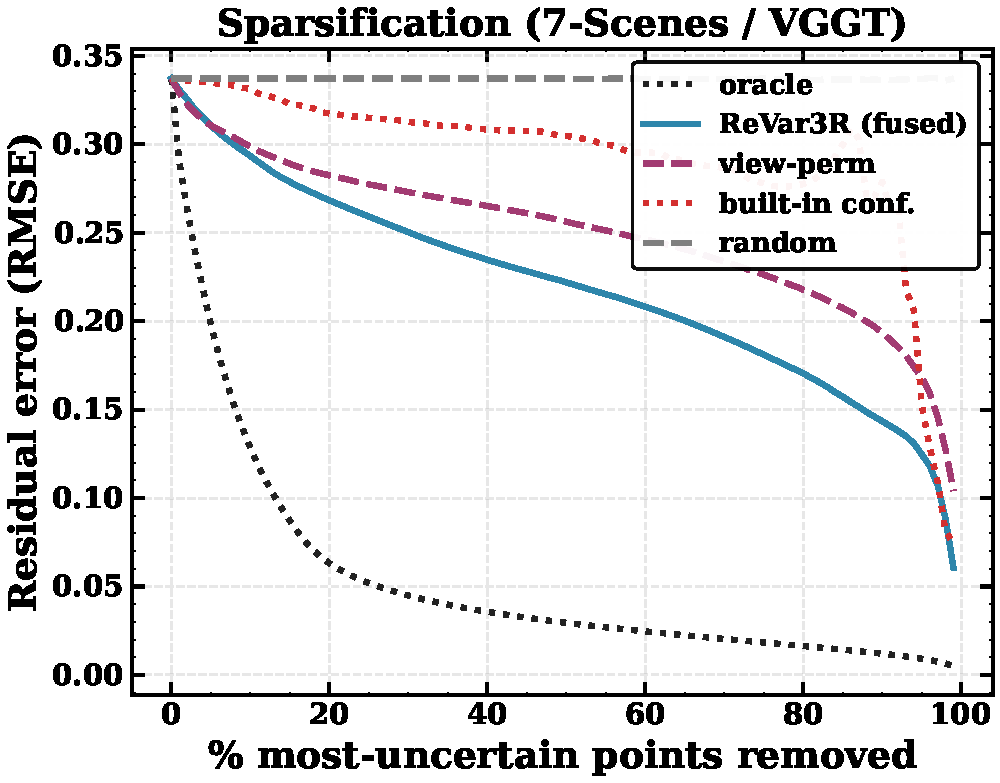
\includegraphics[width=\linewidth]{rq2_sparsification_clean_vggt_sevenscenes.pdf}
  \caption{\textbf{Sparsification} (\vggt/7-Scenes). \trustr's residual-error drop tracks the
  \emph{oracle}; the built-in confidence barely beats \emph{random}. The gap between the curves is the
  \ause.}
  \label{fig:spars}
\end{figure}

\subsection{Main result: \trustr\ beats the built-in confidence}
\label{sec:exp-main}

Throughout, \trustr\ denotes a single headline estimator: the held-out, inverse-\ause-weighted rank
fusion of the two perturbation families \emph{together with} the model's own built-in confidence
(\Cref{sec:method}); the perturbation-only and equal-weight variants are reported beside it
(\Cref{sec:ablations}). \Cref{tab:rq2}, \Cref{fig:spars}, and \Cref{fig:cross} report the headline.
Across the full $3{\times}4{=}12$ grid, \trustr\ significantly reduces \ause\ in \textbf{9 of 12}
cells (by $3\text{--}36\%$; $p$ from $3{\times}10^{-2}$ to $9{\times}10^{-10}$), lifting Spearman
from $\le{+}0.07$ to as high as $+0.49$, and it \emph{restores the sign} of the correlation where it
was negative (\vggt/BlendedMVS $-0.12\to+0.43$, \mastr/DTU $-0.10\to+0.23$).

\paragraph{The headline is the out-of-distribution result.} On ETH3D, where the built-in confidence
flat-lines (Spearman $\approx 0$ for all three models), \trustr\ wins for \emph{every} architecture
($-3$ to $-10\%$, $p\le 6{\times}10^{-3}$): a training-free signal survives the very shift that breaks
the model's own confidence. We are careful about what carries this. Out-of-distribution it is the
\emph{perturbation} signal, not the fusion machinery: the simplest input-noise baseline (MC) already
matches or beats the built-in-augmented fusion on ETH3D, and a perturbation-only fusion is marginally
stronger there (the held-out fusion pays a small OOD cost for admitting the correlation-collapsed
built-in confidence as a candidate family; \Cref{sec:abl-fusion}). Both still clear the built-in
confidence---the deployed baseline---which is the claim we make.

\paragraph{The wins are predicted by mis-calibration---and so are the non-wins.} The three non-wins
are exactly the BlendedMVS column: the models' own training corpus, where the built-in confidence is
\emph{already} well-calibrated and \trustr\ correctly adds little. This coupling is stronger and more
honest than blanket superiority---indeed a perfect $12/12$ would be \emph{suspicious}, implying the
method ``improves'' even where the confidence is already good, which would suggest it is fitting
noise. (On BlendedMVS a large pooled $\Delta$ and the paired $p$ can look discordant---\vggt\ shows a
$-48\%$ pooled reduction yet $p{=}0.19$---because this rendered corpus mixes heterogeneous source
scans: the built-in confidence is locally sensible but globally mis-scaled, so its \emph{per-set}
\ause\ ($0.38$ for \vggt) is far below its \emph{pooled} $0.78$, and the per-set Wilcoxon we report
correctly factors that cross-scene scaling out; \Cref{sec:primer-metrics}.) \Cref{fig:qual} shows the
maps: \trustr's uncertainty mirrors true-error structure where the built-in confidence does not.

\begin{table*}[tb]
  \centering\small
  \adjustbox{max width=\textwidth}{\input{tables/tab2_rq2}}
  \caption{\textbf{Main result} (\ause\dn, mean over 3 seeds). \trustr\ has lower \ause\ in $10/12$
  cells ($\Delta<0$) and a \textbf{significant} win (paired-Wilcoxon $p<0.05$ \emph{and} lower \ause;
  \best{bold}) in \textbf{9 of 12}, \emph{including OOD for all three models}. The three non-wins are
  the BlendedMVS column---the models' own training corpus, where the built-in confidence is already
  well-calibrated.}
  \label{tab:rq2}
\end{table*}

\begin{figure}[tb]
  \centering
  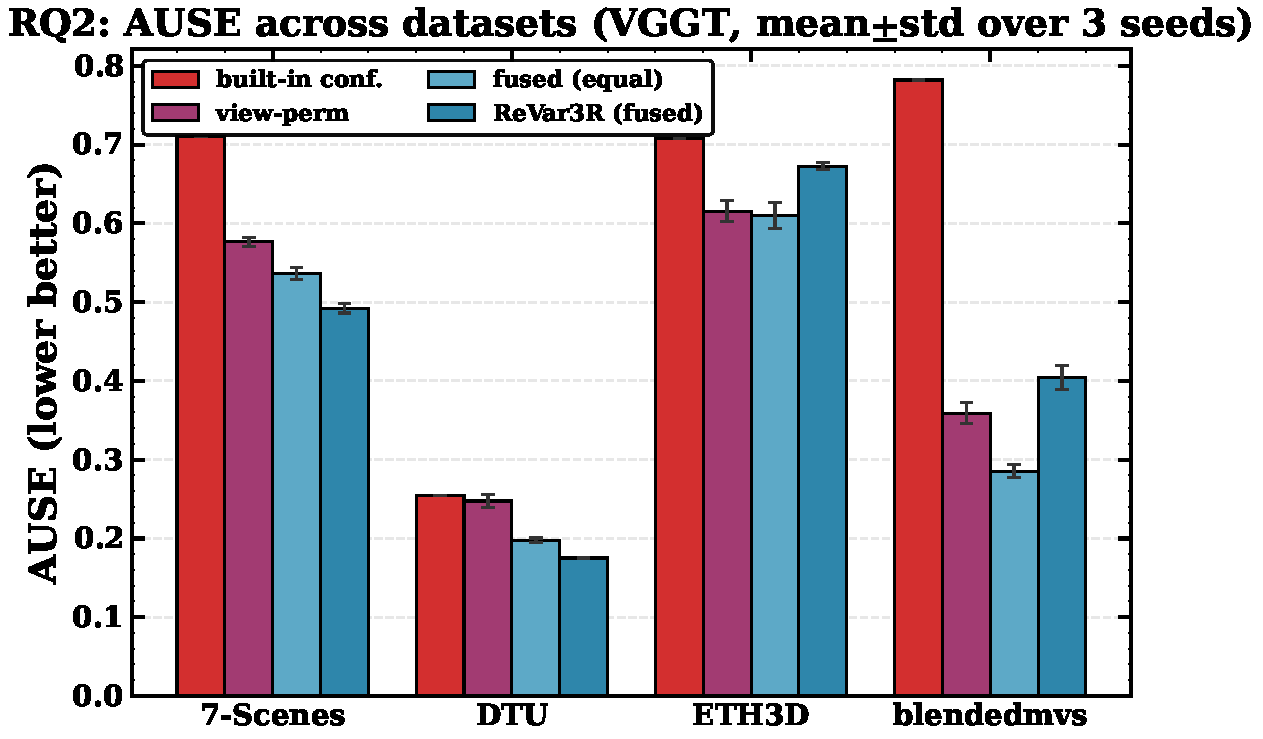
\includegraphics[width=\linewidth]{rq2_cross_dataset.pdf}
  \caption{\textbf{Cross-dataset \ause} (\vggt, mean$\pm$std over 3 seeds). The built-in confidence
  (red) is the weakest signal on all four datasets and \trustr\ (held-out weighted fusion) the
  strongest; the margin is largest on BlendedMVS and OOD ETH3D, where the built-in confidence is
  mis-calibrated ($\rho<0$ and $\approx 0$).}
  \label{fig:cross}
\end{figure}

\begin{figure*}[tbp]
  \centering
  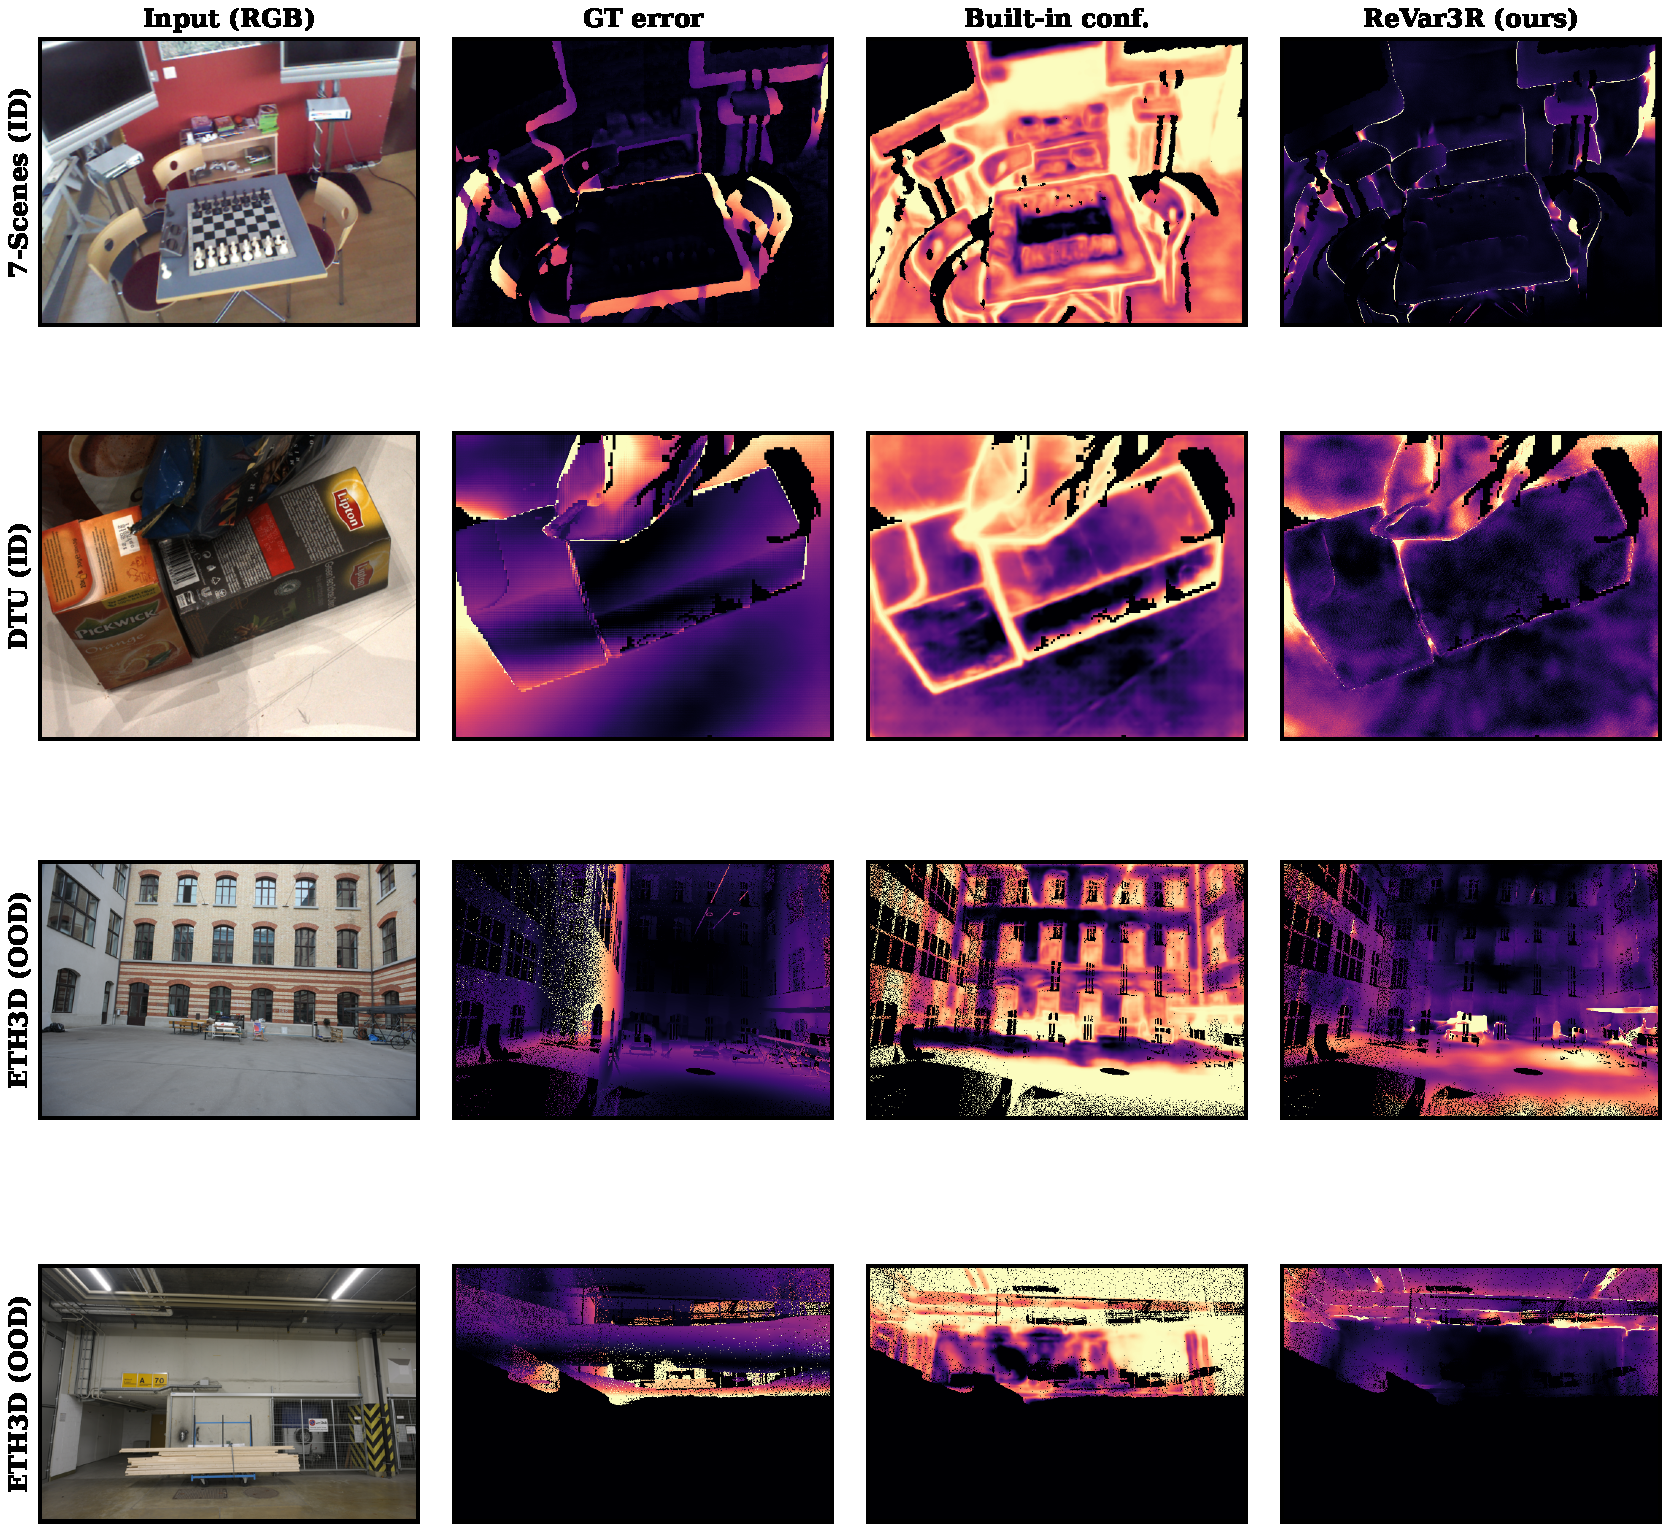
\includegraphics[width=0.92\linewidth]{qualitative.pdf}
  \caption{\textbf{Qualitative} (\vggt). For a reference view: input, GT error, built-in confidence
  (as uncertainty), and \trustr. \trustr\ highlights the genuinely-erroneous regions (object
  boundaries, textureless and far-depth areas); the built-in confidence is diffuse and, OOD,
  uncorrelated. Brighter $=$ more uncertain.}
  \label{fig:qual}
\end{figure*}

\subsection{The win holds across architectures, which govern the signal}
\label{sec:exp-arch}

\Cref{fig:bymodel} and \Cref{tab:rq2} show \trustr\ beats the built-in confidence on all three
architectures on 7-Scenes and ETH3D---the reference-dependent \vggt\ and \mastr\ ($-36\%$) and the
permutation-equivariant \pii\ ($0.509\to0.359$, $-29\%$ on 7-Scenes; $-10\%$ OOD). The gains are
architecture-agnostic \emph{where the built-in confidence is mis-calibrated}; on \pii's
already-well-calibrated BlendedMVS it correctly does not improve.

Crucially, the architecture governs \emph{which} perturbation carries the signal, exactly as the
gauge analysis (\Cref{sec:primer-gauge}) predicts. For the reference-dependent \vggt/\mastr,
view-permutation is the strongest single perturbation; for the equivariant \pii, where re-ordering is
inert by construction, the signal comes from photometric jitter and view-\emph{subset}, and the
held-out weighting drives the inert shuffle's weight to $\approx 0$ automatically. The
\emph{fitted fusion weight}---high on the view-perm family for \vggt/\mastr, near zero for
\pii---reads this architectural fact out cleanly, with no special-casing in the pipeline
(full per-signal breakdown in \Cref{sec:abl-fusion}).

\begin{figure}[tb]
  \centering
  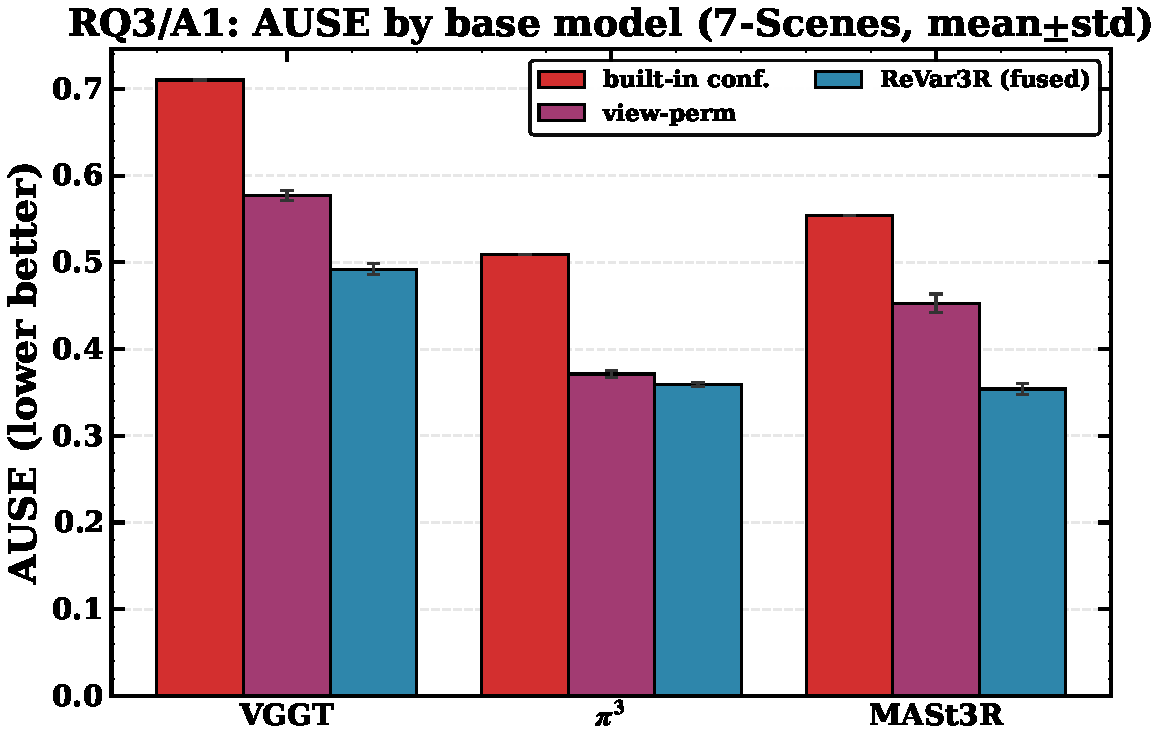
\includegraphics[width=\linewidth]{rq3_by_model.pdf}
  \caption{\textbf{By base model} (7-Scenes). \trustr\ beats the built-in confidence on \vggt, \pii,
  and \mastr.}
  \label{fig:bymodel}
\end{figure}

\subsection{The signal is epistemic, not in the features}
\label{sec:probe}

If \trustr\ merely re-discovered information already present in one forward pass, a model trained to
read that information should match it. We test this directly. We train a small MLP probe on the
model's \emph{frozen} features (final-aggregator patch tokens, bilinearly sampled to pixels) to
regress per-point error, on held-out scenes with a leakage-free 2-fold split---the strongest
\emph{trained} reference. \Cref{tab:probe} shows \trustr\ \emph{matches or beats this trained probe on
\ause\ on every dataset}. On 7-Scenes the probe cannot even beat the built-in confidence
($0.79$ versus $0.70$)---the error signal is \emph{not} linearly decodable from a single forward
pass---yet \trustr\ reaches Spearman $+0.29$ where the probe reaches $+0.09$.

The interpretation is mechanistic: the usable signal is \emph{consistent with epistemic
input-sensitivity}, visible only when the model is re-run under perturbations, not a static feature
decodable in one pass. This is the empirical core of the paper's conceptual claim
(\Cref{sec:method-idea}). We are careful not to overclaim: on DTU the probe \emph{does} decode real
signal ($\rho{=}0.56$) and \trustr\ still wins the sparsification \ause, but the probe is a
\emph{reasonable}, not maximal, trained reference (one backbone, a single feature tap, a small MLP);
a stronger decoder---spatial context, multi-layer features---might recover more. This is therefore
\emph{evidence for} the epistemic interpretation, not a proof of an upper bound.

\begin{table}[tb]
  \centering\small
  \adjustbox{max width=\columnwidth}{\input{tables/tab3_probe}}
  \caption{\textbf{\trustr\ vs.\ a trained probe} on the model's frozen features (\ause\dn, Spearman).
  Training-free \trustr\ matches/beats the trained probe everywhere; on 7-Scenes the probe cannot
  beat the built-in confidence.}
  \label{tab:probe}
\end{table}

\subsection{Downstream utility: uncertainty-gated multi-view fusion}
\label{sec:exp-fusion}

A better ranking should translate into a better cloud. When the per-view point maps are fused into one
cloud and the least-trusted points are dropped, \trustr\ selects the wrong points far better than the
built-in confidence (\Cref{fig:fusion}, \Cref{tab:fusion}): at $10\%$ removed it is near-oracle
($0.029$ versus built-in $0.034$\,m on 7-Scenes; $4.10$ versus $4.81$\,mm on DTU), and on DTU it
preserves far more completeness---at $50\%$ removed, confidence-filtering destroys coverage
($20.4$\,mm) while \trustr\ keeps it intact ($9.7$\,mm). This is a concrete, geometry-level payoff for
the better ranking. We report it as an \emph{in-distribution} utility: on OOD ETH3D the fusion gain is
null on \emph{both} accuracy and completeness (all signals $\approx 0.90$\,m accuracy and
$\approx 2.3$\,m completeness at every removal fraction), which we state plainly rather than overclaim.

\begin{figure*}[tbp]
  \centering
  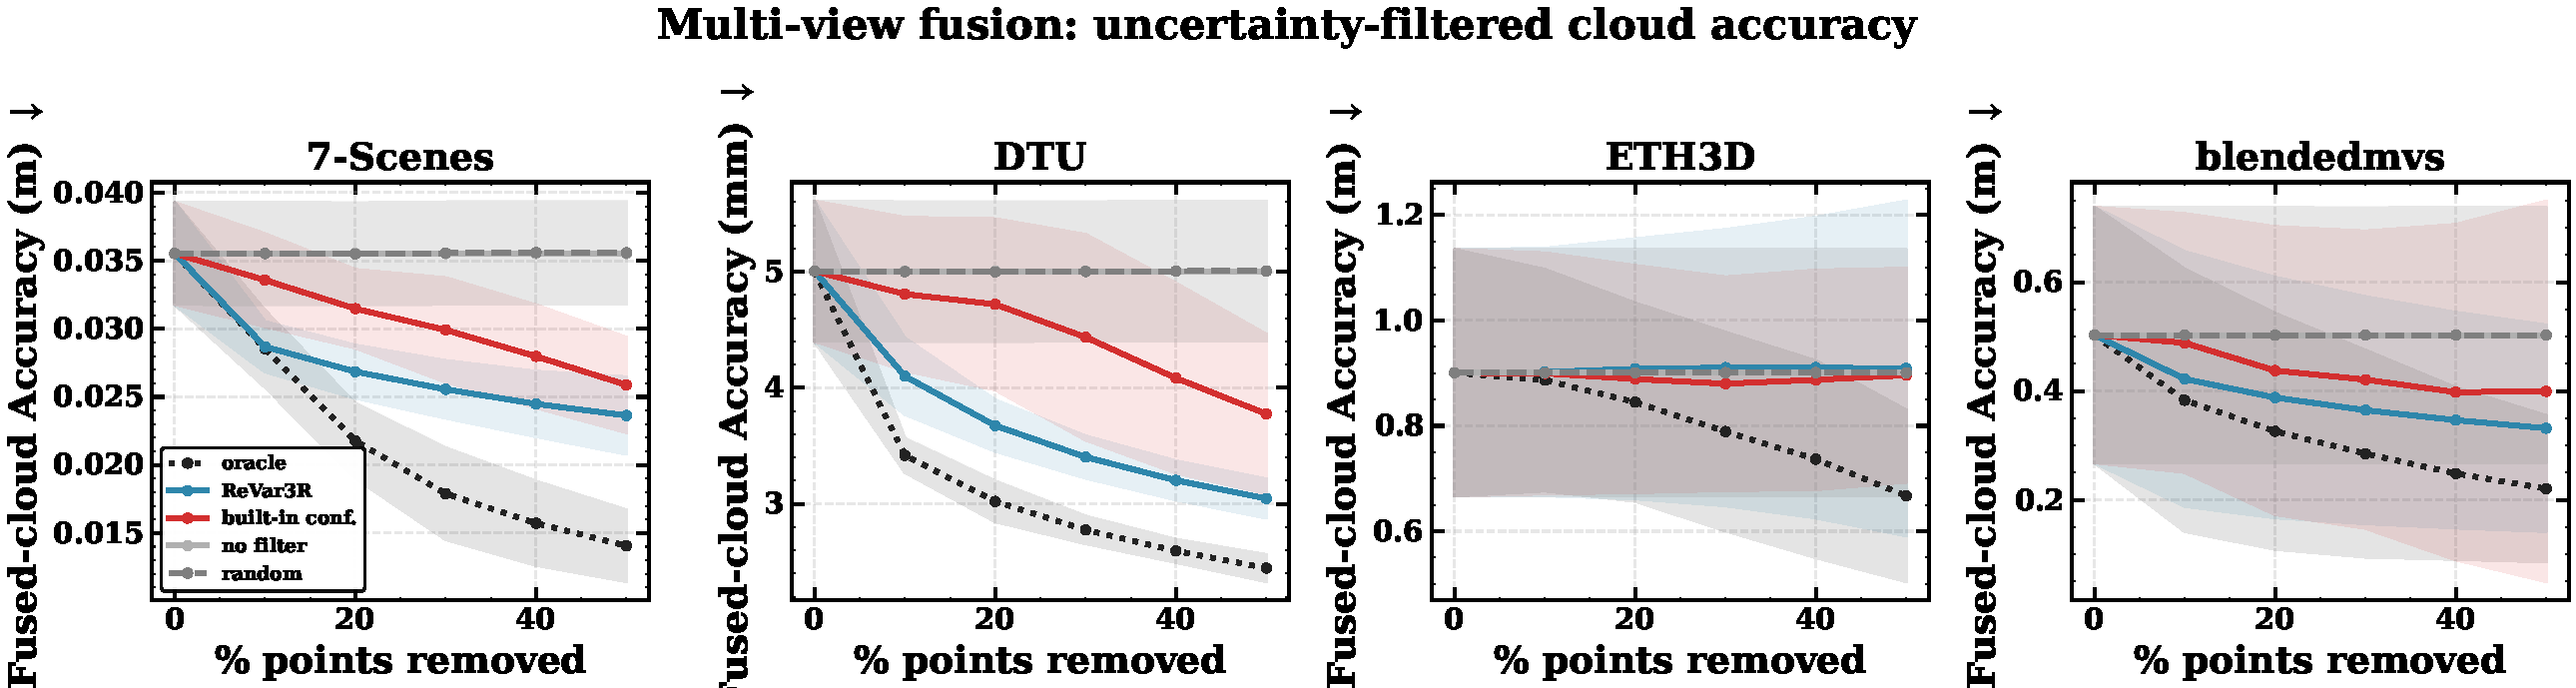
\includegraphics[width=0.96\linewidth]{fusion_accuracy_all.pdf}
  \caption{\textbf{Multi-view fusion.} Fused-cloud Accuracy vs.\ fraction of least-trusted points
  removed. \trustr\ (blue) tracks the oracle on 7-Scenes/DTU; OOD ETH3D shows no gain (stated
  honestly).}
  \label{fig:fusion}
\end{figure*}

\begin{table*}[tb]
  \centering\small
  \adjustbox{max width=\textwidth}{\input{tables/tab5_fusion}}
  \caption{\textbf{Fused-cloud quality} (lower is better). \trustr-filtered fusion is near-oracle and,
  on DTU, preserves much more completeness than confidence-filtering.}
  \label{tab:fusion}
\end{table*}

\subsection{Honest negatives}
\label{sec:exp-neg}

\paragraph{Novel-view synthesis (the null part of H4).} Using \trustr\ to filter 3D Gaussian-Splatting
initialization gives \emph{no} PSNR advantage (all signals within $\sim 0.4$\,dB; random competitive).
This is consistent with our thesis: NVS quality is dominated by appearance/aleatoric factors that the
long per-scene optimization absorbs, not the epistemic geometry uncertainty \trustr\ captures. We
therefore lead the downstream story with multi-view fusion, and report the NVS null plainly
(Appendix~\ref{app:negatives}).

\paragraph{A falsified hypothesis (H3).} We hypothesized that view-permutation disagreement would be a
\emph{stronger} signal for the reference-dependent \vggt\ than for the equivariant \pii. It is not:
relative to each model's built-in confidence, view-perm helps \pii\ at least as much (its gain comes
through leave-one-out \emph{subset} rather than shuffle). The architecture shapes the signal, but not
in the hypothesized direction; we report the characterization (\Cref{sec:exp-arch}), not the original
claim, and analyze the reversal in Appendix~\ref{app:negatives}. Reporting it is the point: a reliability
study that hid its own falsified prediction would undercut its own credibility.

\section{Ablations in depth}
\label{sec:ablations}

An \emph{ablation} changes exactly one design choice and re-runs the identical evaluation, so any
change in the score is attributable to that one choice (\emph{ceteris paribus}). Unless noted, the
single-knob ablations are on \vggt/7-Scenes and scored by \ause\ (lower is better; recall from
\Cref{sec:primer-metrics} that \ause\ is rank-only, so calibration cannot move it---calibration is
scored by \ece). Every number is read directly from the result CSVs. \Cref{tab:ablfull} and
\Cref{fig:ablgrid} give the full A1--A12 sweep; we then discuss the two design-defining knobs in
depth, summarize the rest, and finish with the calibration (\Cref{sec:abl-calib}) and fusion
(\Cref{sec:abl-fusion}) studies.

\begin{table*}[t]
\centering\small
\adjustbox{max width=\textwidth}{\input{tables/tab_ablation_full}}
\caption{Full single-knob ablation A1--A12 (\vggt/7-Scenes; \ause\dn\ except A8, which is \ece\dn).
\best{Bold} marks the best level per factor. Alignment (A7) is the dominant knob
($0.715\!\to\!0.496$); calibration (A8) moves only \ece\ ($0.296\!\to\!0.094$, $\sim 3\times$);
held-out fusion weights (A12) $\approx$ equal ($0.585$ vs.\ $0.586$).}
\label{tab:ablfull}
\end{table*}

\begin{figure*}[t]
  \centering
  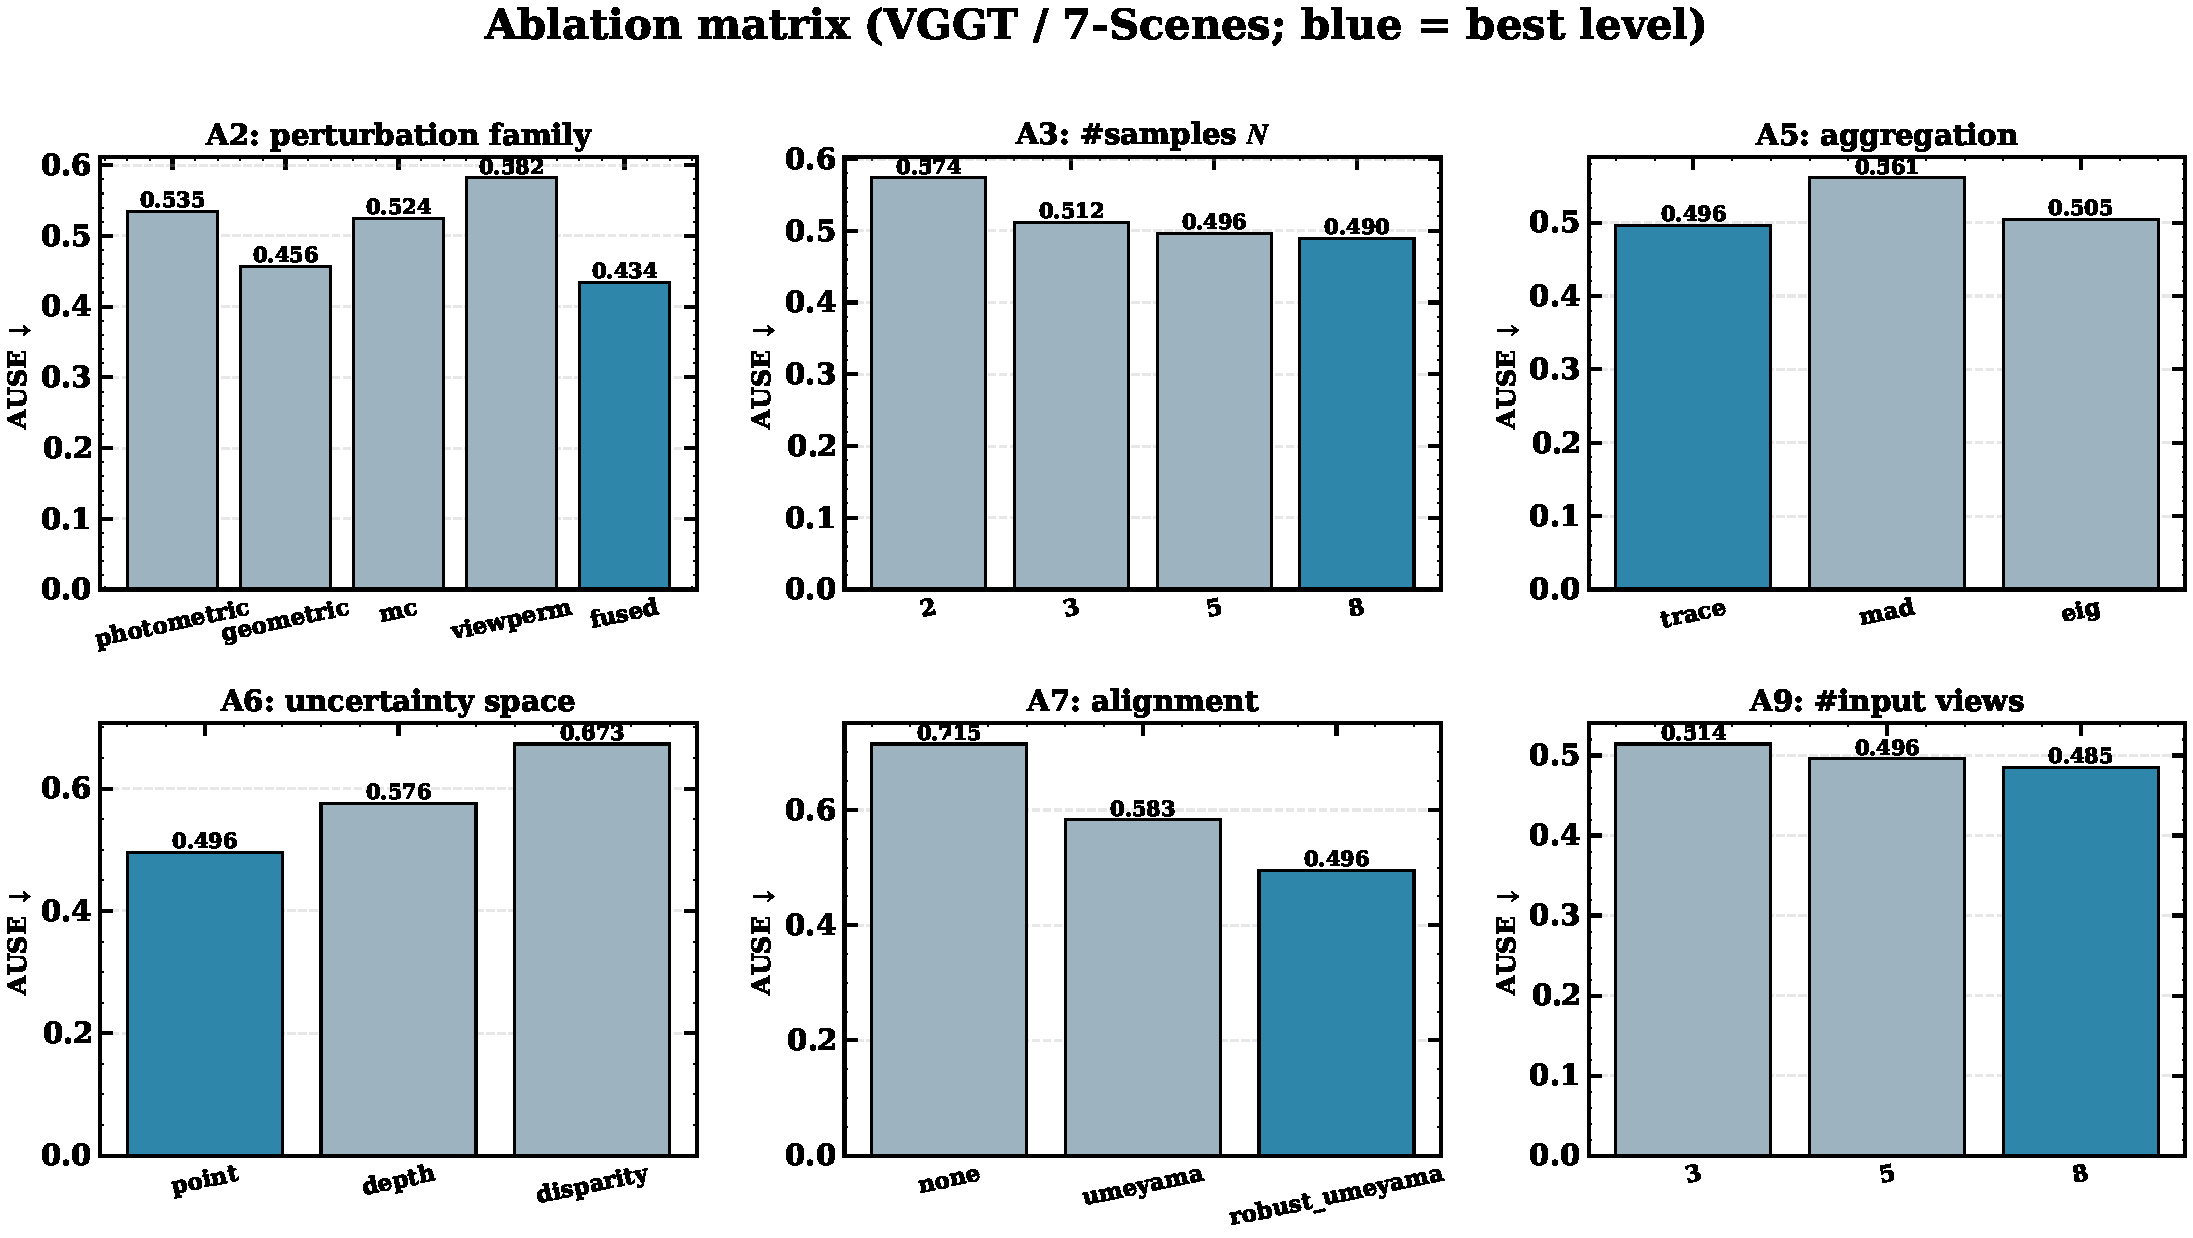
\includegraphics[width=0.95\textwidth]{ablation_grid.pdf}
  \caption{Ablation matrix (\vggt/7-Scenes; \ause\dn, blue $=$ best level per factor). Single-knob
  sweeps over perturbation family, sample count $N$, aggregation, uncertainty space, alignment, and
  input views.}
  \label{fig:ablgrid}
\end{figure*}

\subsection{The two design-defining knobs}
\label{sec:abl-standouts}

\paragraph{A7 --- alignment is the technical crux ($0.715\to0.583\to0.496$).} This is a $0.219$
absolute swing from worst to best---larger than any other knob, and larger than the gap between
\trustr\ and the built-in confidence itself. \emph{Why no alignment is near-random} ($0.715$): when
input views are permuted, \vggt/\mastr\ re-express the whole cloud in a different frame (rotation,
translation, \emph{and} global scale, since they lack metric scale). Without alignment the per-point
``spread'' is dominated by these \emph{common-mode} frame offsets---identical for every point---which
swamp the genuine, point-specific disagreement, giving an almost-flat, useless uncertainty.
\emph{Plain Umeyama} ($0.583$) removes the global offset, so the residual spread is mostly real
disagreement. \emph{Robust Umeyama} ($0.496$) additionally stops the worst-disagreeing
points---exactly the ones we want to flag---from tilting the fit and smearing their error onto the
good points. This row is the empirical content of the paper's central conceptual claim: in 3D the
runs live in incompatible frames, so alignment-before-variance is the method, not bookkeeping.

\paragraph{A8 --- calibration, measured in \ece\ not \ause\ ($0.296\to0.094$).} Calibration is a
monotone remap and \ause\ is rank-invariant, so calibration \emph{cannot} change \ause\ by
construction; measuring it in \ause\ would misleadingly show ``no effect.'' Its job is to make the
magnitude honest (a stated $90\%$ interval really contains $90\%$ of errors), scored by \ece, fit on
one half and evaluated on the held-out half. \emph{None} ($0.296$) is badly mis-calibrated.
\emph{Temperature} ($0.372$)---a single global multiplier---is \emph{worse than none}, because this
raw single-family uncertainty is mis-\emph{shaped}, not merely mis-\emph{scaled}, and one scalar
cannot fix a nonlinear distortion. \emph{Isotonic} ($0.094$)---an arbitrary monotone
Pool-Adjacent-Violators curve---matches the shape of the error distribution and cuts \ece\ roughly
$3\times$ while preserving ranks (hence \ause).

\subsection{The remaining knobs, briefly}
\label{sec:abl-rest}

\begin{itemize}[leftmargin=1.4em,itemsep=2pt,topsep=2pt]
\item \textbf{A1 (base model).} \trustr\ generalizes: \vggt\ $0.496$ and \pii\ $0.380$, both far below
their built-in baselines ($0.710$ and $0.509$). \pii's lower absolute \ause\ is an easier base signal,
not a \vggt\ failure.
\item \textbf{A2 (perturbation family).} photo $0.535$, geom $0.456$, mc $0.524$, viewperm $0.582$,
\emph{fused} $0.434$: the fusion beats every single family---no one perturbation is best.
\item \textbf{A3 (samples $N$).} $0.574/0.512/0.496/0.490$ for $N{=}2/3/5/8$: a sharp gain to $N{=}5$,
then flat ($5\to8$ moves \ause\ by $0.0006$). $N{=}5$ is the cost/quality knee; $N{=}3$ already
recovers $\approx 93\%$ of the gain.
\item \textbf{A4 (photometric strength).} $0.532/0.535/0.543$ for low/med/high: a spread of $\approx
0.01$---essentially insensitive, so the recipe is not a tuned hyper-parameter.
\item \textbf{A5 (aggregator).} trace $0.496$, MAD $0.561$, eig $0.505$: trace-variance is best.
\item \textbf{A6 (uncertainty space).} point $0.496$, depth $0.576$, disparity $0.673$: measuring
spread in native 3D-point space is materially better than in depth or disparity.
\item \textbf{A9 (input views).} $0.514/0.496/0.485$ for $3/5/8$ views: more views help with
diminishing returns; $5$ is the default knee.
\item \textbf{A11 (view-perm mode).} shuffle $0.582$ vs.\ subset $0.581$: a tie on the
reference-dependent \vggt\ (both expose reference instability). For the equivariant \pii, shuffle is
inert and subset is the one that works (\Cref{sec:exp-arch}).
\item \textbf{A12 (fusion weighting).} equal $0.586$ vs.\ learned $0.585$: close in-distribution; the
value of the held-out weighting shows up against the built-in baseline once it is a fusion family
(\Cref{sec:abl-fusion}).
\item \textbf{A13/A14 (downstream).} the 3DGS-initialization null and the multi-view-fusion win,
already reported in \Cref{sec:exp-fusion,sec:exp-neg}.
\end{itemize}

\subsection{Calibration generalizes across the grid, and needs almost no ground truth}
\label{sec:abl-calib}

\Cref{fig:reliability} (A8) is the raw single-family signal on one cell. \Cref{tab:q2ece} reports the
regression \ece\ of the \emph{headline fused} signal for all twelve cells, before and after the
isotonic step (held-out 2-fold over view-sets). With a single global scale the fused signal is already
moderately calibrated (\ece\ $0.04$--$0.15$); the isotonic map reduces \ece\ further where it is
largest---the out-of-distribution ETH3D cells (e.g.\ \pii/ETH3D $0.072\to0.037$) and the higher-error
DTU cells (\mastr/DTU $0.146\to0.103$)---and is approximately neutral on the already-low cells.

\begin{figure}[tb]
  \centering
  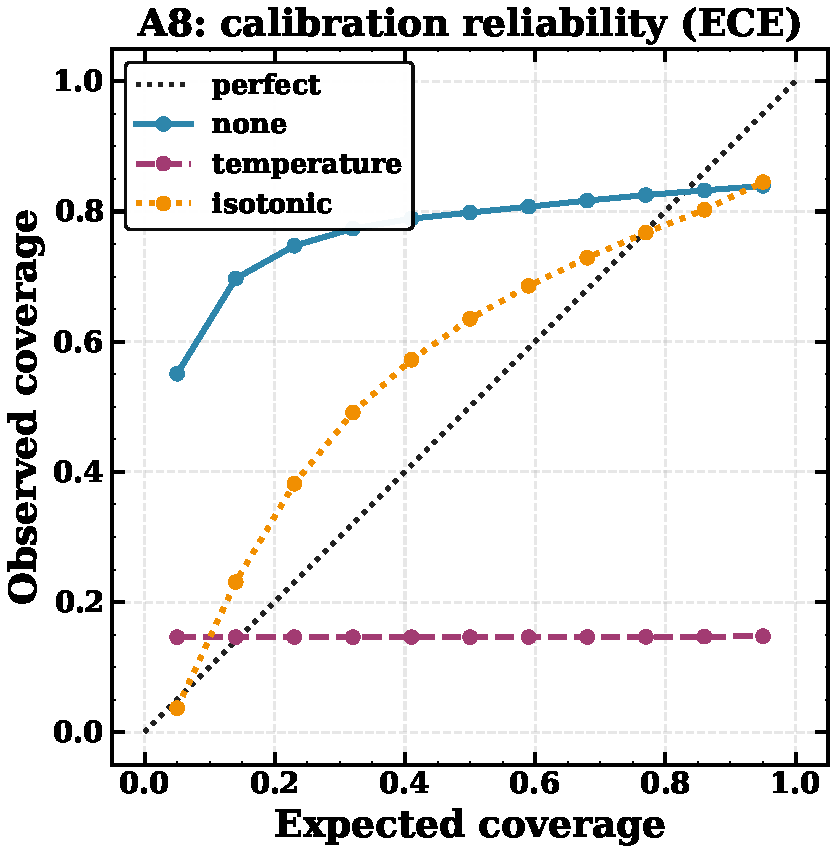
\includegraphics[width=0.8\linewidth]{A8_reliability.pdf}
  \caption{Calibration reliability (A8): the isotonic mapping brings observed coverage onto the
  diagonal, cutting \ece\ $\sim 3\times$.}
  \label{fig:reliability}
\end{figure}

\begin{table*}[tb]
\centering\small
\adjustbox{max width=\textwidth}{\input{tables/tab_q2_ece}}
\caption{Per-cell regression \ece\dn\ of the headline fused signal: a single global scale (``raw'')
vs.\ a held-out isotonic map. Isotonic helps most on the out-of-distribution and higher-error cells.}
\label{tab:q2ece}
\end{table*}

How much ground truth does calibration actually need? \Cref{tab:q6} answers directly. The registered
cross-run spread is a faithful \emph{rank} predictor of error---all \ause\ and the fusion use---but it
systematically \emph{under}-estimates the absolute error (it measures epistemic input-sensitivity,
not total error), so used as a raw $\sigma$ it is maximally mis-calibrated (\ece\ $\approx 0.50$). A
\emph{single} global scale, estimable from any small labelled sample, removes this bias and recovers
most of the calibration (\ece\ $0.50\to0.14$ on average); a small held-out isotonic split refines it
to $0.08$. The method's ground-truth requirement thus reduces to \emph{one scalar} for absolute
coverage---the ranking, \ause, and fusion are entirely ground-truth-free.

\begin{table*}[tb]
\centering\small
\adjustbox{max width=\textwidth}{\input{tables/tab_q6_calib}}
\caption{\textbf{Calibration needs only one scalar of ground truth.} Regression \ece\dn\ of the metric
perturbation uncertainty under three calibrations: raw $\sigma$ (no GT), a single global scale (one
number of GT), and a held-out isotonic map. One scalar removes the systematic under-confidence.}
\label{tab:q6}
\end{table*}

\subsection{Fusion: equal vs.\ held-out weighting, and is the headline circular?}
\label{sec:abl-fusion}

\Cref{tab:allsig} reports \ause\ for \emph{every} signal across all twelve cells---the built-in
confidence, the MC baseline, the two standalone \trustr\ families, and the two fusions. Two patterns underpin the main
text. First, view-permutation is the strongest single family on the reference-dependent \vggt/\mastr\
and weaker (though not inert) on \pii, where its signal comes from leave-one-out subset rather than
shuffle. Second, the held-out weighted fusion and the equal-weight fusion are close but not identical.

\begin{table*}[tb]
\centering\small
\adjustbox{max width=\textwidth}{\input{tables/tab_allsignals}}
\caption{Per-signal \ause\dn\ (mean over 3 seeds) for all 12 cells. Columns: built-in confidence;
MC/latent-noise baseline; the two standalone \trustr\ families (photometric, view-perm); and the
equal-weight and held-out-weighted fusions. \best{Bold} marks the best (lowest) signal in each row.}
\label{tab:allsig}
\end{table*}

\paragraph{Equal vs.\ held-out weighting.} \Cref{tab:fuserob} contrasts the two directly. Against the
built-in baseline, the held-out weighting wins $9$ of $12$ cells to equal fusion's $8$; crucially it
\emph{recovers} \pii/DTU---the one cell the perturbation families alone regress---which equal fusion
turns into a regression. Equal fusion is, in turn, marginally stronger on the out-of-distribution
ETH3D cells, where admitting the correlation-collapsed built-in confidence as a candidate slightly
dilutes the perturbation signal. The mechanism is structural: under shift the built-in confidence is
collapsed in rank correlation ($\rho\approx 0$) yet only \emph{moderately} worse in \ause\ than the
perturbation families, and because the inverse-\ause\ weight is soft it cannot drive a moderately-worse
family to zero---so the collapsed built-in still earns roughly a fifth to a quarter of the weight and
dilutes the cleaner perturbation signal. Two facts keep this in perspective: \emph{(i)} both fusions
still beat the built-in confidence on every OOD cell, so the headline OOD result is invariant to the
fusion choice; and \emph{(ii)} the weighting earns its keep in-distribution (the \pii/DTU recovery)
and never collapses far below a genuinely-good confidence. We therefore adopt the held-out weighting
as the principled, leakage-free default, and note that under \emph{known} domain shift the simpler
choice---drop the built-in family and use a perturbation-only fusion---is marginally better.

\begin{table*}[tb]
\centering\small
\adjustbox{max width=\textwidth}{%
\begin{tabular}{llcc}
\toprule
Model & Dataset & Equal fusion & \trustr\ (held-out $+$ built-in) \\
\midrule
\vggt & 7-Scenes & 0.537 & 0.492 \\
\vggt & DTU & 0.198 & 0.175 \\
\vggt & ETH3D (OOD) & 0.610 & 0.673 \\
\vggt & BlendedMVS & 0.286 & 0.405 \\
\pii & 7-Scenes & 0.351 & 0.359 \\
\pii & DTU & 0.340 & 0.231 \\
\pii & ETH3D (OOD) & 0.480 & 0.616 \\
\pii & BlendedMVS & 0.234 & 0.281 \\
\mastr & 7-Scenes & 0.404 & 0.354 \\
\mastr & DTU & 0.320 & 0.352 \\
\mastr & ETH3D (OOD) & 0.600 & 0.644 \\
\mastr & BlendedMVS & 0.377 & 0.308 \\
\bottomrule
\end{tabular}}
\caption{Equal vs.\ held-out weighted fusion (\ause\dn, mean over 3 seeds). The held-out weighting
adds the built-in confidence as a fusion family: it wins more cells against the built-in baseline
($9$ vs.\ $8$) and recovers \pii/DTU, while equal fusion is marginally stronger OOD.}
\label{tab:fuserob}
\end{table*}

\paragraph{Is the comparison circular?} Including the built-in confidence as a fusion family invites
the worry that beating that same confidence is rigged. It is not. \Cref{tab:q3decouple} removes the
built-in family from the fusion entirely: a held-out, inverse-\ause\ rank fusion of the two
\emph{perturbation} families alone still significantly beats the built-in confidence on $8$ of $12$
cells. Re-adding the built-in family as a third candidate lifts this to $9/12$, the single additional
cell being \pii/DTU. The training-free perturbation signal therefore carries the result on its own;
the built-in family helps only where it is genuinely informative, and the three non-wins are exactly
the BlendedMVS column, the models' own training corpus.

\begin{table*}[tb]
\centering\small
\adjustbox{max width=\textwidth}{\input{tables/tab_q3_fusion}}
\caption{\textbf{Decoupling the headline from the baseline} (\ause\dn, held-out fusion, mean over 3
seeds). \best{Bold} marks a significant per-set win over the built-in confidence. Perturbation-only
fusion (\emph{no} built-in) already wins $8/12$; adding the built-in family reaches $9/12$, recovering
\pii/DTU. The three non-wins are exactly the BlendedMVS training corpus.}
\label{tab:q3decouple}
\end{table*}

\section{Discussion and limitations}
\label{sec:discussion}

\trustr\ rests on a simple principle---a frozen model's \emph{disagreement with itself} under
equivalent inputs is an epistemic signal---made to work in 3D by registering runs before measuring
variance. The probe experiment (\Cref{sec:probe}) suggests \emph{why} it beats the model's own
confidence: that confidence is a static function of one forward pass, whereas reliability here lives
in the model's \emph{sensitivity} to the input, which only a re-run exposes. The contribution is
conceptual rather than a perturbation recipe: \emph{(i)} in 3D, self-disagreement is meaningful only
after each run's gauge is removed---\emph{naive} variance is near-random ($0.72$ vs.\ $0.50$
\ause)---so robust registration \emph{before} variance is load-bearing; and \emph{(ii)} the usable
reliability signal is epistemic input-sensitivity, invisible to a probe on a single forward pass.
Together they turn a frozen reconstructor into a self-assessing one with no training.

\paragraph{Limitations.} We state the scope honestly; several of these are the natural next problems.

\begin{enumerate}[label=(\roman*),leftmargin=1.8em,itemsep=2pt,topsep=2pt]
\item \textbf{Cost.} The estimator costs $\le 10$ forward passes; for latency-critical use this is the
main overhead, though the $N{=}5$ knee (and the cheaper $N{=}3$ point) keeps it modest.
\item \textbf{Not every perturbation is exactly geometry-preserving.} Photometric jitter and view
\emph{shuffling} leave the scene unchanged, but leave-one-out \emph{subsetting} removes constraints
and can alter which surfaces are co-visible, so its disagreement conflates input-sensitivity with a
coverage change. Empirically the two view-perm modes are nearly indistinguishable on the
reference-dependent models (A11: $0.582$ vs.\ $0.581$ \ause), and subsetting is decisive only for the
permutation-equivariant \pii, whose output is invariant to a shuffle; we therefore read its subset
signal as a conservative lower bound on input-sensitivity rather than a pure geometric probe. Richer
training-free perturbations---a more diverse photometric/geometric TTA set, or activation-space noise
injected into the frozen backbone---are a natural complementary family to fuse, and a plausible route
to closing the residual out-of-distribution gap to input-noise baselines such as MC.
\item \textbf{The fully-specified estimator is not zero-GT.} Its held-out fusion \emph{weights} and
its isotonic \emph{calibration} are each fit on a small per-domain held-out split (never the test
points). What \emph{is} GT-free is the per-point uncertainty \emph{signal}---each perturbation family,
and the parameter-free \emph{equal} fusion, a close (and OOD-stronger) alternative to the
weighting---and calibration's GT need reduces to essentially \emph{one global scalar}
(\Cref{sec:abl-calib}). A fully GT-free variant (equal fusion $+$ a single global scale) is therefore
available at a small cost; only absolute coverage benefits from a labelled split.
\item \textbf{Metric-scale data.} Our datasets are metric-scale with reliable GT; in-the-wild scenes
without GT are future work.
\item \textbf{The downstream win is geometric.} It is multi-view fusion, not photometric novel-view
synthesis (\Cref{sec:exp-neg}).
\item \textbf{A complement, not a replacement.} \trustr\ helps precisely where the built-in confidence
is mis-calibrated (out-of-distribution and several in-distribution cells) and correctly adds nothing
where it is already well-calibrated, so the gain is conditional---which we view as evidence the signal
is real rather than a universal claim.
\item \textbf{It measures procedural variance, not systematic bias.} \trustr\ measures epistemic
uncertainty as \emph{input-sensitivity}---the model's procedural, local variance under
perturbation---so it flags where the model is \emph{unstable}, but not a \emph{systematic bias} where
the model is stably and confidently wrong (cross-run variance $\approx 0$ yet error large); such bias
lies outside the reach of any perturbation-variance estimator. Our gains fall on the input-sensitive
failure modes, consistent with the standard decomposition of epistemic uncertainty into model bias
versus procedural variance~\cite{epistemic_incomplete}.
\end{enumerate}

A natural next step is to use per-point \trustr\ uncertainty to gate points in SLAM/SfM back-ends and
feed-forward Gaussian-Splatting pipelines, and---to reach the bias component above---to complement the
perturbation signal with a learned or cross-model estimator that can detect stable-but-wrong
predictions.

\section{Conclusion}
\label{sec:conclusion}

We showed that the built-in confidence of frozen feed-forward 3D foundation models is an
\emph{uneven} uncertainty---weak in-distribution, $\rho{\approx}0$ out-of-distribution, and
\emph{anti-correlated} on several cells---and introduced \trustr, a training-free, single-GPU
estimator that registers perturbed runs before measuring variance. Across three models and four
datasets \trustr\ significantly reduces \ause\ in \textbf{9 of 12} cells (by $3\text{--}36\%$),
\emph{wins out-of-distribution for all three architectures} where the model's own confidence
collapses, \emph{exceeds a probe trained on the model's frozen features}---evidence that the signal
is \emph{consistent with} epistemic input-sensitivity---and delivers a near-oracle in-distribution multi-view-fusion gain,
with honest negatives reported. We hope the OOD characterization and the training-free benchmark are a useful
reliability layer for the fast-growing \emph{family of systems built on DUSt3R/VGGT-style point-map models}.

The estimator is, deliberately, the simplest thing that works: re-run a frozen model, align, and
look at where it disagrees with itself. Its main limitation is also conceptual---input-perturbation
variance measures the model's \emph{procedural} sensitivity, not a systematic bias where the model is
stably and confidently wrong---and the natural next steps (a learned single-pass amortization of the
signal, a bias-aware complement, and uncertainty-gated SLAM/Gaussian-Splatting back-ends) all build on
the same primitive.


\appendix
\section{Protocol and reproducibility}
\label{app:repro}

\paragraph{Hardware / software.} All experiments run on a single NVIDIA RTX 5060 Ti (16\,GB,
Blackwell sm\_120), PyTorch 2.11 + CUDA 12.8, bfloat16, on a host capped at ${\sim}7$\,GiB RAM. A full
\trustr\ uncertainty map is $N{=}5$ forward passes per family; peak VRAM $\approx 11$\,GB.

\paragraph{Models.} \vggt-1B (\texttt{facebook/VGGT-1B}), \pii\ (\texttt{yyfz233/Pi3X}), and \mastr\
(metric checkpoint). \mastr\ is pairwise; we obtain a common frame by \emph{anchored-pairwise}
inference (pair view-0 with each other view and read every point map in view-0's frame), avoiding
global alignment. View-0 anchors every pair and is thus the most constrained view; perturbation
variance is computed identically for anchor and non-anchor views, and we report per-view results
including the anchor.

\paragraph{Configuration.} $5$ input views, $N{=}5$ samples, $518$\,px, robust-Umeyama alignment
(IRLS, $5$ iterations, Cauchy weights, drop worst $10\%$, fit on an $8$k-point subsample;
Algorithm~\ref{alg:align}), trace-variance aggregation in 3D-point space, isotonic calibration fit per
model on a held-out split, held-out inverse-\ause\ rank fusion of the photometric and view-perm
families together with the built-in confidence.

\paragraph{Perturbations.} Photometric: brightness/contrast/gamma and colour jitter, mild Gaussian
noise and blur (medium strength; strength is ablated, \Cref{sec:abl-rest}). View-perm: random
re-ordering and leave-one-out/subset resampling of the input views.

\paragraph{Correspondence and masking.} Uncertainty is a per-pixel quantity in each input view's own
image grid, so correspondences across the $N$ perturbed runs are pixel identity within a view, not
feature matches. Before aggregation each perturbed prediction is mapped back to the canonical view
order and pixel grid: photometric/MC jitter leave the grid unchanged (identity); the geometric family
applies its stored inverse affine; the view-permutation family re-indexes the views, filling any view
dropped by a leave-one-out sample with NaN so it never contributes to that pixel's variance. The $N$
canonicalized point maps are registered to the first sample by the same robust similarity and reduced
by NaN-aware trace-variance; a pixel with fewer than two finite samples is set to the per-map maximum
(a conservative ``maximally uncertain'' fill). For error, the prediction is aligned to GT by a
gauge-freeing robust similarity over pixels with valid GT only; a view with fewer than $50$ valid
pixels is dropped, and the same $\ge\!50$-correspondence floor guards every similarity/scale fit (it
falls back to identity below it). Built-in confidence enters as uncertainty $\max(c)-c$.

\paragraph{Evaluation.} Per-point error is computed after a gauge-freeing robust similarity alignment
of the prediction to GT. Every number is the mean over $3$ seeds; significance is a paired Wilcoxon
signed-rank test over view-sets. Each figure reports the oracle (error-sorted) and random references.

\paragraph{A verified metric/geometry core.} Before any real result is trusted, the metrics and
geometry are proven on synthetic data with known answers (fixed seed, runnable unit tests): the
oracle ranking yields \ause\ $\approx 0$; a useless signal yields $\approx 0$ \aurg; the Umeyama
solver inverts a clean transform to $<10^{-6}$; the robust variant recovers the transform with $10\%$
gross outliers (the exact A7 failure mode); the aggregator recovers an injected spread; and rank
fusion is provably immune to a family rescaled by $10^6$ (the precise reason rank fusion replaced an
earlier z-normalized fusion that collapsed on DTU). Every number rests on a metric/geometry core
independently verified on inputs with known ground truth.

\paragraph{Single source of truth.} All knobs live in one \texttt{base.yaml}; every paper table is
generated directly from per-run CSVs (no hand-typed numbers). Code, configs, and figure/table scripts
will be released.

\section{Formal metric definitions}
\label{app:metrics}

This appendix gives the formal counterparts of the intuitions in \Cref{sec:primer-metrics}. Let $e_i$
be the per-point error and $U_i$ the predicted uncertainty over $P$ valid points.

\paragraph{Sparsification / \ause.} Sort points by $U_i$ descending; for fraction $r\in[0,1]$ removed,
$s(r)$ is the RMSE of $e_i$ over the kept points. The \emph{oracle} curve $o(r)$ sorts by the true
$e_i$. Then $\ause = \int_0^1 |s(r)-o(r)|\,dr$, normalized by the no-removal error so scenes are
comparable. Lower is better, and it is invariant to any monotone re-scaling of $U$.

\paragraph{\aurg.} $\int_0^1 (s_{\mathrm{rand}}(r)-s(r))\,dr$, the area between the random-removal
curve and the method curve; higher is better.

\paragraph{Correlation.} Spearman $\rho$ between $U_i$ and $e_i$ (rank correlation; reported) and
Pearson.

\paragraph{Regression \ece.} Following~\cite{kuleshov}, treat the error as zero-mean Gaussian with
standard deviation $U_i$; for target coverage $q$, measure the empirical fraction of points whose
$|e_i|$ falls in the predicted central interval, and report the mean $|\text{observed}-q|$ over
$q\in[0.05,0.95]$.

\paragraph{Fused-cloud Accuracy / Completeness.} After gauge-freeing alignment, Accuracy is the mean
nearest-neighbour distance from kept predicted points to the GT cloud; Completeness is the mean
nearest distance from GT to the kept predicted cloud (mm for DTU, m otherwise).

\paragraph{\ause-MAE.} Besides the headline \ause-RMSE we also report \ause\ under an $L_1$
(mean-absolute) error aggregation; \Cref{tab:ausemae} shows \trustr's ranking advantage is preserved
under this variant.

\begin{table}[h]
\centering\small
\adjustbox{max width=\columnwidth}{\input{tables/tab_ause_mae}}
\caption{\ause\ under $L_1$ error aggregation (\dn). \trustr\ vs.\ the built-in confidence.}
\label{tab:ausemae}
\end{table}

\section{Statistical detail}
\label{app:perscene}

All significance tests in the paper are paired Wilcoxon signed-rank tests computed over individual
\emph{view-sets} (which span the constituent scenes of each dataset: 7-Scenes chess/fire/heads; DTU
object scans; ETH3D courtyard/electro/office/pipes/terrace), so the reported $p$-values already
account for per-scene variation. The seed standard deviations in \Cref{tab:rq2} (e.g.\
$0.490{\pm}0.006$ on 7-Scenes; $0.640{\pm}0.009$ on OOD ETH3D) quantify run-to-run stability; the
held-out weighted and equal-weight fusions are comparably stable, and the perturbation-only fusion
wins the identical $8/12$ cells (\Cref{sec:abl-fusion}).

\section{Additional sparsification curves}
\label{app:curves}

\Cref{fig:morecurves} shows sparsification curves for \vggt\ and \pii\ beyond the main 7-Scenes panel
(\Cref{fig:spars}); in both, \trustr\ tracks the oracle and clearly separates from the built-in
confidence and random references.

\begin{figure}[h]
  \centering
  \begin{subfigure}{0.49\linewidth}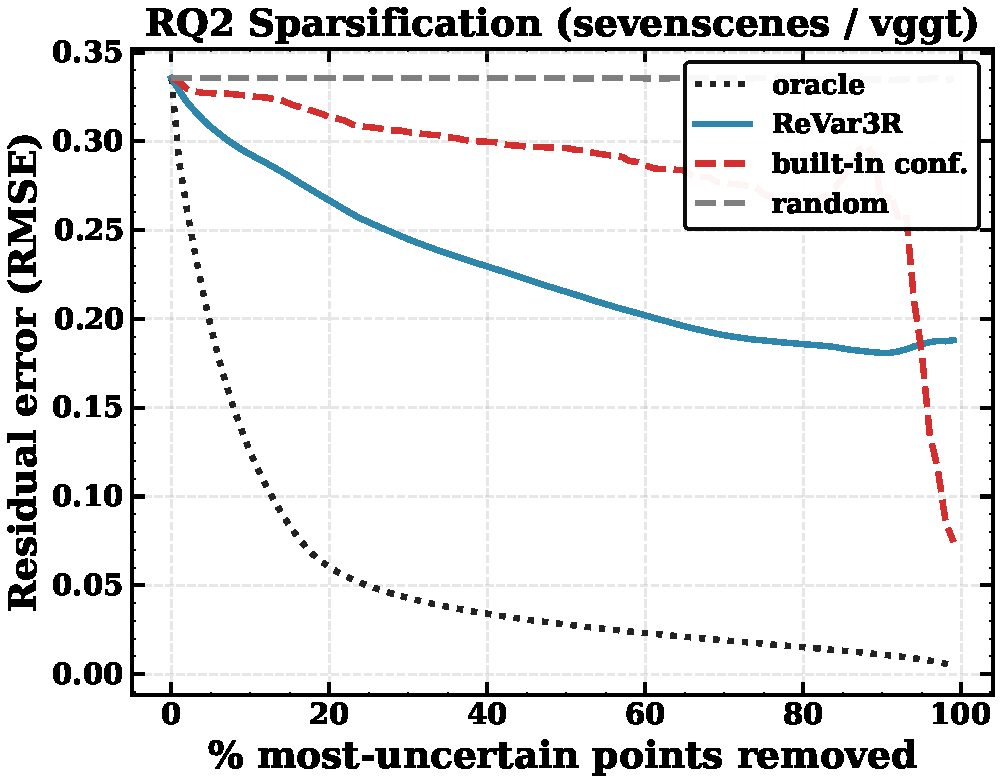
\includegraphics[width=\linewidth]{rq3_sparsification_vggt.pdf}
    \caption{\vggt}\end{subfigure}\hfill
  \begin{subfigure}{0.49\linewidth}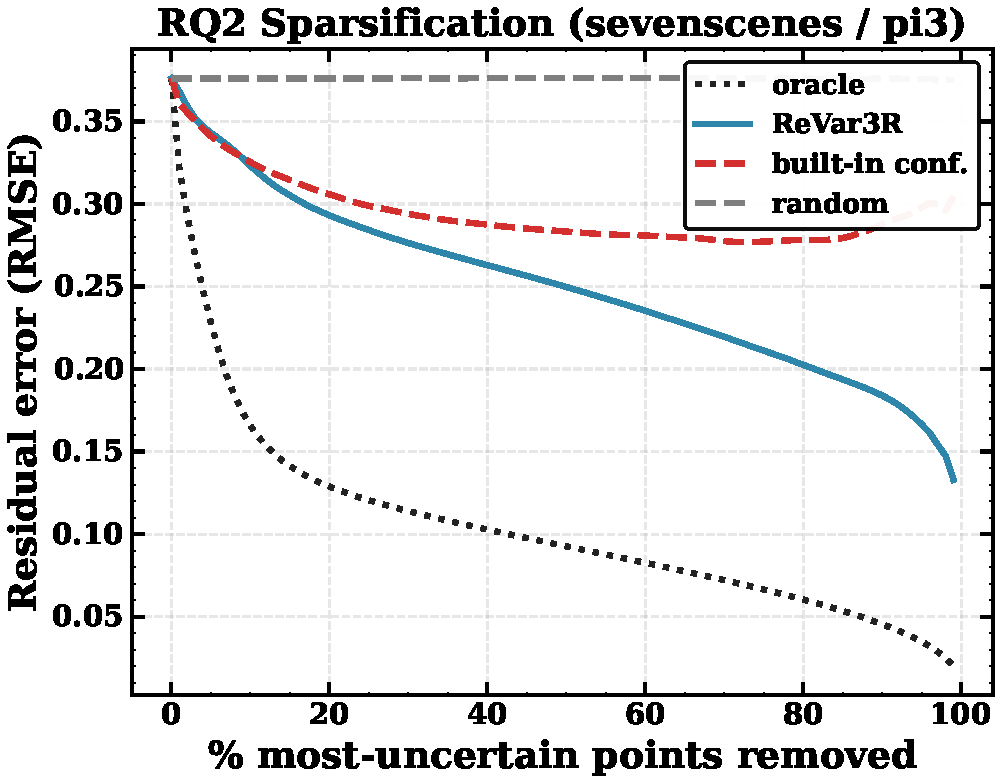
\includegraphics[width=\linewidth]{rq3_sparsification_pi3.pdf}
    \caption{\pii}\end{subfigure}
  \caption{Additional sparsification curves (7-Scenes).}
  \label{fig:morecurves}
\end{figure}

Beyond 7-Scenes, \Cref{fig:morecurves2} shows the curves on DTU, on the out-of-distribution ETH3D
set, and for the third architecture (\mastr): \trustr\ tracks the oracle in-distribution and, OOD,
still separates from the (here near-flat) built-in confidence.

\begin{figure*}[t]
  \centering
  \begin{subfigure}{0.32\textwidth}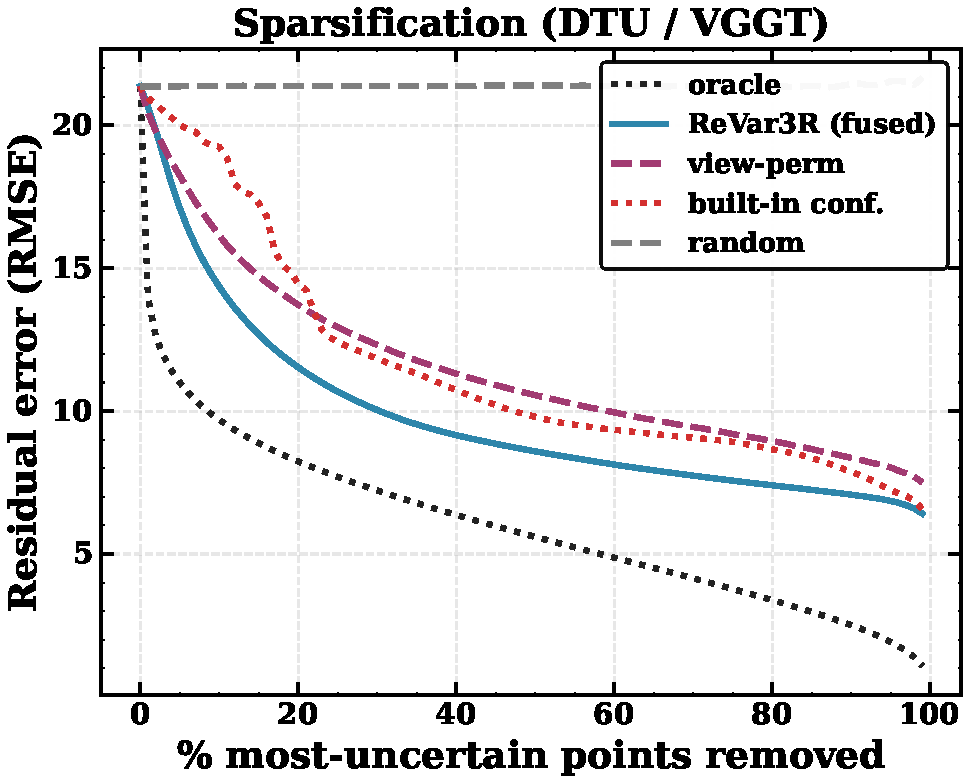
\includegraphics[width=\linewidth]{rq2_sparsification_clean_vggt_dtu.pdf}
    \caption{\vggt\ / DTU}\end{subfigure}\hfill
  \begin{subfigure}{0.32\textwidth}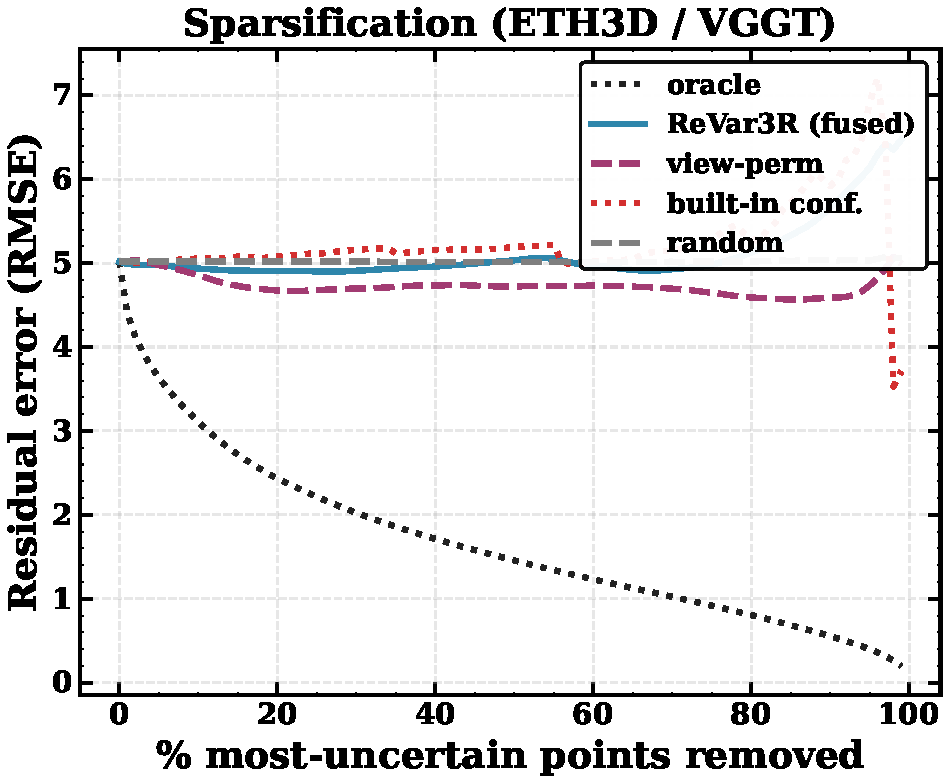
\includegraphics[width=\linewidth]{rq2_sparsification_clean_vggt_eth3d.pdf}
    \caption{\vggt\ / ETH3D (OOD)}\end{subfigure}\hfill
  \begin{subfigure}{0.32\textwidth}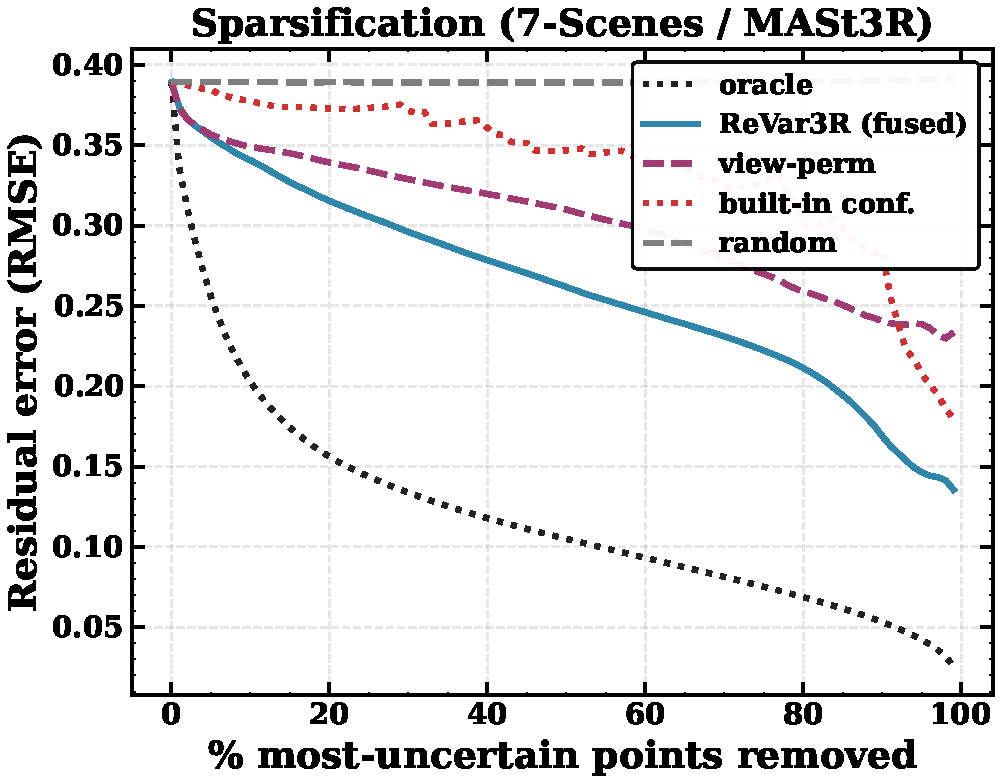
\includegraphics[width=\linewidth]{rq2_sparsification_clean_mast3r_sevenscenes.pdf}
    \caption{\mastr\ / 7-Scenes}\end{subfigure}
  \caption{Per-dataset and per-model sparsification (DTU, OOD ETH3D, and the third architecture,
  \mastr). \trustr\ (fused) tracks the oracle and beats the built-in confidence; OOD the gain is
  smaller but the curve still separates.}
  \label{fig:morecurves2}
\end{figure*}

\section{Additional qualitative results}
\label{app:qual}

\Cref{fig:qual} (main text) shows in-distribution and out-of-distribution scenes with the input, GT
error, built-in confidence, and \trustr\ uncertainty for a reference view. \trustr\ concentrates
uncertainty on object boundaries, textureless regions, and far-depth areas---where feed-forward point
maps are genuinely least reliable---whereas the built-in confidence is diffuse and, out-of-distribution,
uncorrelated with the error. The ETH3D rows illustrate the harder OOD regime, where the gain is
smaller but the spatial correspondence to true error is still visible.

\section{Negative results in full}
\label{app:negatives}

\paragraph{Novel-view synthesis (the null part of H4).} We initialize 3D Gaussian
Splatting~\cite{gsplat} from the predicted point map, optionally filtering or weighting points by each
uncertainty signal, optimize for a fixed budget, and render a held-out view. \Cref{fig:nvs} shows no
signal yields a meaningful PSNR advantage (all within $\sim 0.4$\,dB; random competitive). The
per-scene optimization (the Gaussians migrate and split until they fit the training views regardless
of where they started) absorbs the initialization differences, and NVS quality is dominated by
appearance/aleatoric factors rather than the epistemic geometry uncertainty \trustr\ captures. We
therefore report multi-view fusion (\Cref{sec:exp-fusion}) as the downstream utility. Reporting this
null prevents over-claiming and motivates the task where the signal is \emph{not} washed out.

\begin{figure}[h]
  \centering
  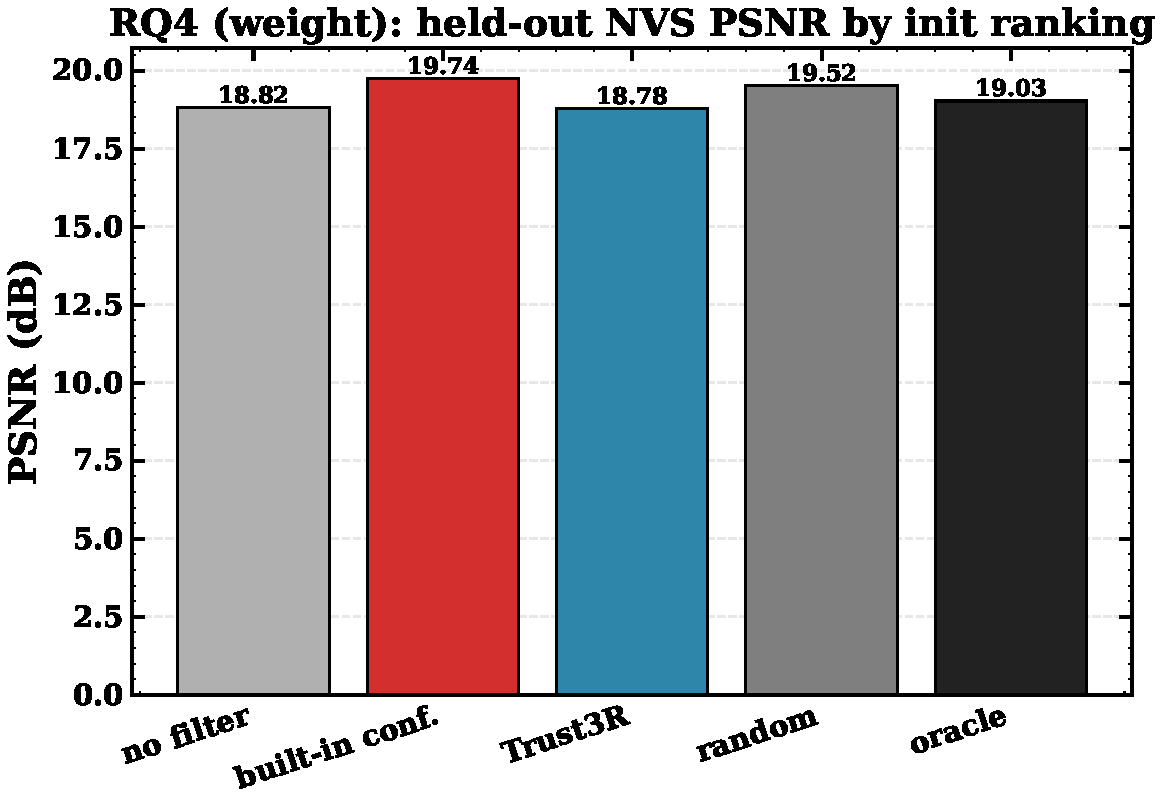
\includegraphics[width=0.85\linewidth]{rq4_psnr_weight_vggt.pdf}
  \caption{Uncertainty-weighted 3DGS-init NVS: held-out PSNR by ranking signal. No method separates;
  an honest null.}
  \label{fig:nvs}
\end{figure}

\begin{table}[h]
\centering\small
\adjustbox{max width=\columnwidth}{\input{tables/tab_downstream}}
\caption{Held-out NVS quality (weighted init) by ranking signal. No signal---including
\trustr---wins on PSNR\up/SSIM\up/LPIPS\dn; the gaps are within noise.}
\label{tab:downstream}
\end{table}

\paragraph{Falsified hypothesis (H3).} We hypothesized that view-permutation disagreement would be a
stronger signal for the reference-dependent \vggt\ than for the permutation-equivariant \pii. Relative
to each model's built-in confidence, the view-perm estimator reduces \ause\ by $19\%$ for \vggt\ but
$27\%$ for \pii---the opposite of the prediction. A plausible mechanism is that subset resampling perturbs the shared latent geometry
regardless of reference-dependence, and \pii's better-calibrated global point map retains more order
sensitivity. We report the characterization, not the original claim---the honest negative is itself
part of the contribution.

\section{Notation and terminology}
\label{app:glossary}

A compact reference for the recurring terms (\Cref{sec:primer}).

\begin{description}[leftmargin=1.1em,itemsep=1.5pt,topsep=3pt,style=unboxed]
\item[Frozen model.] A pretrained network we run but never modify; there is no training anywhere in the method.
\item[Point map.] Per-pixel predicted 3D coordinates $(x,y,z)$; the model's main output.
\item[Built-in confidence.] A per-pixel number the model already emits, trained as a loss weight---not a calibrated error estimate.
\item[Perturbation / TTA.] A small change to the input (``test-time augmentation'') that should not change the true 3D.
\item[Geometry-preserving.] A perturbation that leaves the real 3D unchanged, so any output change is the model's fault, not induced.
\item[Gauge / similarity.] The seven degrees of freedom---scale (1), rotation (3), translation (3)---that the output is only defined up to.
\item[Reference-dependent.] A model (\vggt, \mastr) whose gauge is anchored on a chosen first view; contrast with permutation-equivariant.
\item[Permutation-equivariant.] A model (\pii) whose output does not depend on the input view order, so a shuffle is inert.
\item[Alignment / registration.] Undoing the gauge: scaling/rotating/shifting one run onto another so they share one frame.
\item[Umeyama.] The closed-form least-squares algorithm for the best similarity transform between two point sets~\cite{umeyama}.
\item[IRLS / robust fit.] Iteratively re-weighted least squares: fitting while down-weighting outliers so a few bad points cannot ruin the fit.
\item[Trace-variance.] Our raw uncertainty: the RMS distance of the $N$ registered runs from their per-pixel mean (the spread).
\item[Calibration.] Rescaling raw uncertainty so its magnitude is meaningful (a stated ``$90\%$ interval'' really contains $90\%$ of errors).
\item[Isotonic regression.] The best monotone (order-preserving) fit; our calibration map, computed by Pool-Adjacent-Violators.
\item[Held-out fusion.] Combining perturbation families (and the built-in confidence) with weights fit on a held-out split, never on the scored points.
\item[Epistemic uncertainty.] The model's own ignorance; reducible, and detectable by probing the model and watching it become unstable.
\item[Aleatoric uncertainty.] Irreducible noise in the data (sensor noise, blur, genuine ambiguity); not what \trustr\ targets.
\item[\ause\ ($\downarrow$).] Area Under the Sparsification Error; the headline metric: how well uncertainty \emph{ranks} error vs.\ an oracle. Rank-only.
\item[\aurg\ ($\uparrow$).] Area gained over the random-removal baseline; $\approx 0$ for a no-skill signal.
\item[Spearman $\rho$ ($\uparrow$).] Rank correlation between uncertainty and error; $+1$ perfect, $0$ useless, negative actively misleading.
\item[\ece\ ($\downarrow$).] Expected Calibration Error; whether the uncertainty \emph{magnitudes} are honest. The only metric calibration moves.
\item[Oracle / random.] The best-possible ranking (sort by true error) and the no-skill baseline; every plot is bracketed by these.
\item[ID / OOD.] In-distribution (data like training) / out-of-distribution (a domain shift that stresses the model).
\item[View-set.] The unit of evaluation: a handful of overlapping images of one scene.
\item[MC baseline.] A simple input-noise stand-in for MC-dropout (the checkpoints have no dropout); a baseline, not a tuned competitor.
\end{description}


{\small
\bibliographystyle{ieeenat_fullname}
\bibliography{refs}
}

\end{document}
